\documentclass{article}
\usepackage{amsmath}
\usepackage{array,multirow}
\usepackage{amsfonts}
\usepackage{graphicx}
\usepackage{geometry}
\usepackage{cite}
%======================================%
%              Graphics                %
%======================================%
\usepackage{graphicx}
\graphicspath{{images/}}
\usepackage[font=small,labelfont=bf]{caption} % Required for specifying captions to tables and figures
\usepackage[subrefformat=parens]{subcaption}
\usepackage {tikz}
\usetikzlibrary{calc}


\geometry{margin=1in} % Adjust the margins as needed

\begin{document}

\newpage
%%%%%%%%%%%%%%%%%%%%%%%%%%%%%%%%%%%%%%%%%%%%%%%%%%%%%%%%%%%%%%%%
%                          Cover                               %
%%%%%%%%%%%%%%%%%%%%%%%%%%%%%%%%%%%%%%%%%%%%%%%%%%%%%%%%%%%%%%%%

\title{		
{Numerical Schemes for problems of Phase Seperation}\\ 

		{\small National Technical University of Athens} \\~\\\
		{
\includegraphics{ntua.jpg}}\\
		{\small Thesis submitted for M.Sc. Program in Computational Mechanics}\\ 
		{\small supervised by M.Kavousanakis} 
	  }
	  
\author{Chantzaras Lampros}
\date{\today}
\maketitle




\newpage 

\ % The empty page

\newpage

\section*{Acknowledgments}

I would like to take the opportunity to thank my thesis supervisor, Mihalis Kavousanakis,
Assistant Professor of the School of Chemical Engineering at the National Technical University
of Athens, for his insightful advice and guidance throughout the course of this thesis.\\

A special thanks also goes to my younger brother Giannis, for his patience and his willingess to devote serious amount of time and his specific knowledge of computer science, to help me with every implementation aspect. His effort was crucial to completing this thesis.\\

Finally, I want to thank all my colleagues and the Professors of this Joint Postgraduate Studies Program for our collective interaction throughout the course of the program was essential for developing my understanding on the core subjects of the program.


\newpage
\section*{Abstract}
The Cahn--Hilliard (CH) equation is a mathematical model of the process of phase separation in a binary alloy \cite{Cahn1958FreeEO}. 

Initially proposed in view of applications to mettalurgy and materials science to study phase separation and coarsening in materials, such as binary alloys, polymers, and liquid crystals, also to study the growth and morphology of thin films in material deposition processes, such as epitaxial growth. These applications have been extended to various scientific fields, including spinodal decomposition in the context of statistical mechanics, where it is used to describe the process in which a homogeneous mixture separates into two distinct phases \cite{Cahn1958FreeEO,CAHN1961795}, diblock copolymer, image inpainting, multiphase fluid flows where it can be used to model the behavior of two immiscible fluids, like oil and water, and their interface dynamics, amongst others \cite{BADALASSI2003371}, microstructures with elastic inhomogeneity \cite{0a06993046834526b042d6c742445fc9}, tumor growth simulation \cite{MOHAMMADI2019919}, and topology optimization \cite{article}.\\

In the Cahn-Hilliard equation, the evolution of concentration consists of two stages:  Fast phase separation where the energy decay happens quickly, i.e. on a small time scale, is followed by phase coarsening until the two different phases obtain constant curvature. Fine-scaled phase regions separated by the interface form at the end of the first stage, while the solution reaches an equilibrium state minimizing the energy functional at the end of the second stage.\\

Numerical methods that are developed for the Cahn-Hilliard equation often should take into account the nonlinearity in the system, the presence of the small parameter $\epsilon$ (thickness of the interface), and the different time scales that characterise the concentration evolution. Resolution schemes require proper scaling of numerical parameters, such as the spatial mesh size $h$ and often adaptive time stepping techniques for the time step size $k$, relative to the interaction length $\epsilon$.\\

The aim of this thesis, is to show the effectiveness and the high accuracy of the numerical scheme arising from the the standard conforming mixed finite element formulation of this problem. Three main cases for the boundary conditions  to close the problem are examined, namely the standard (Neumann), the periodic and the specified contact angle conditions. For this work, we consider the domain to be a rectangle and discretize the problem using the standard Lagrange 9-node elements. Then we fully discretize
the problem in time using the implicit backward Euler-method, which is of first order accuracy. The resulting nonlinear algebraic
system for every time step time step is then solved by a Newton-Raphson iteration procedure and during each iteration, a linear system with the
corresponding Jacobian has to be solved. For this linear system the biconjugate gradient method (BiCGStab) method is employed.
\newpage


\tableofcontents
\section{The basic framework of the Phase Field Model}



Here we state the essential considerations for the derivation of the phase field model for the completeness of the work to follow.
For the  interested reader the rigorous derivation of the phase-field model can be found to:  \cite{Elliott1989}. Also an instructive review of the main ways to derive the Cahn-Hilliard equation can be found in [LEE2014216].\\

Consider a binary fluid system consisting of two immiscible viscous fluids,denoted as fluids 1 and 2 under constant temperature, completely occupying a bounded domain $\Omega$ in $\mathbb{R}^2$, with a sufficiently smooth boundary denoted as $\partial\Omega$. The total density of the mixture is defined as $\rho_m = \frac{m}{V}$ is considered constant, $m$ represents the total mass of the mixture in the characteristic volume $V$ (i.e., $m = \int_{\Omega} \rho_m dx$). We assume that the two fluids possess different apparent densities defined as $\rho_i' = \frac{m_i}{V}$ also constans for $i = 1, 2$. We define the apparent densities as $\rho_i'$. These are related to the actual densities $\rho_i = \frac{m_i}{V_i}$ through $\rho_i' = V_{f_i} \rho_i$, where $V_{f_i} = \frac{V_i}{V}$ represent the volume fractions, and $m_i$ represents the masses of the components in $\Omega$, defined as:

\[
m_i = \int_{\Omega} \rho_i' dx,
\]


The total mass $m$ is the sum of the masses of fluids 1 and 2:\\

\[
\rho_m = \rho_1' + \rho_2'
\]

We consider that the interface between the two phases has a thin nonzero thickness characterized by a rapid and smooth transition. The scalar function $\phi$, known as the 'order parameter' is used to represent the two phases and the transition in between.

\[
\phi = \begin{cases}
    1, & \text{in fluid 1}, \\
    -1, & \text{in fluid 2}, \\
    [-1, 1], & \text{in the interfacial region}.
\end{cases}
\]

The cause of the spatial transition of the two materials is consider to be the local surface tension (we assume constant temperature, incompressibility of the fluids and viscosity). Consequently, the total amount of each fluid in $\Omega$ must remain constant and the principles of mass conservation and of the linear momentum of continuum mechanics apply.\\
The function $\phi$ can be thought of as the difference in local mass fraction of the two fluids:

\[
\phi = \frac{\rho_1' - \rho_2'}{\rho_1' + \rho_2'},
\]\\


or equivalently,

\[
\phi dm_i = \rho_1' dm_idV - \rho_2' dm_i dV
\]

By further manipulation, we obtain

\[
\phi \rho_m = \rho_1' \rho_2'
\]

We observe that $\phi \in [-1, 1]$. When $\phi = 1$ or $\phi = -1$, only fluid 1 or 2 exists, respectively. Moreover, recalling the definitions of $\rho_1'$ and $\rho_2'$, we find that

\[
\int_{\Omega} \rho_m \phi dx = \left(\int_{\Omega} \rho_1' dx\right) \left(\int_{\Omega} \rho_2' dx\right) = m_1 m_2 = \text{constant}.
\]

This demonstrates that the definition of $\phi$ ensures the conservation of the concentration difference between the two fluids in $\Omega$. The conservation of the mass of each component across the entire domain imposes the constraint:

\[
\int_{\Omega} \rho_m \phi(x, t) dx = \text{constant}
\]

The relaxation of the order parameter is driven by local minimization of the free energy subject to phase field conservation and as a result, the interface layers do not deteriorate dynamically. The width of the interfacial layer depends on a parameter $\epsilon$ appearing in the system, and as $\epsilon$ tends to zero, the diffuse interface system converges to the corresponding sharp interface one. Initial ideas can be traced back to van der Waals and form the foundation for the phase-field theory for phase transition and critical phenomena. The phase field motion is governed by a bulk field over the entire domain, and it inherits various interesting properties, including the coupling with physical variables (e.g., velocity and pressure in fluids, temperature), indifference to morphological singularities in the interface, physical dissipation, and a global space discretization. The value $E_{\epsilon}(\phi)$ can represent different interfacial energies associated with the phase field. A basic energy functional is given by:

\begin{equation}
E_{\epsilon}(\phi) = \int_{\Omega}\left(\frac{1}{2}|\nabla\phi|^2 + \frac{1}{\epsilon^2}W(\phi)\right)dx
\end{equation}

where $W(\phi)$ is a double-well potential representing the system's tendency to have two different stable phases, and $\epsilon > 0$ is the parameter related to the interface thickness.\\
\begin{equation}
W(\phi) = \frac{1}{4}(\phi^2 - 1)^2 \quad \text{and} \quad f(\phi) = W'(\phi) = (\phi^2 - 1)\phi.
\end{equation}
% FIG1
\begin{figure*}[!b]
\begin{center}
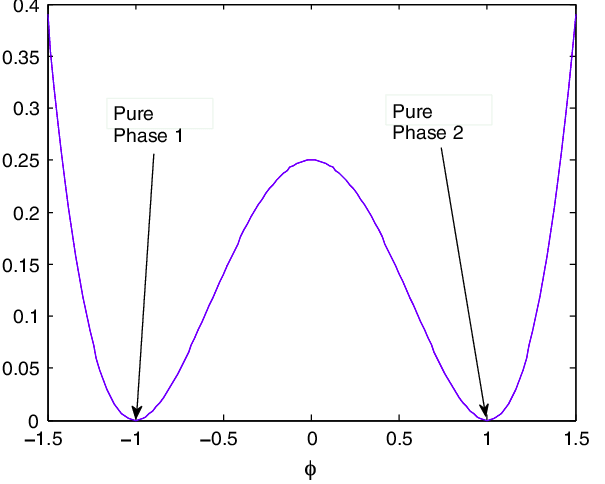
\includegraphics[scale=0.4]{doublewell.png}
\caption{The typical form for the potential}\label{Figure1}
\end{center}
\end{figure*}

There are other possible choices of the double well potential, such as the logarithmic potential, but we concentrate on the Ginzburg-Landau potential for this work. The surface motion can be derived as the dissipation of a phase-field's free energy functional. Here $\frac{\delta E(\phi)}{\delta\phi}$ represents the variational derivative in the $L^2(\Omega)$ or $H^{-1}(\Omega)$ norm for the Cahn-Hilliard equations.

\begin{equation}
\frac{\delta E(\phi)}{\delta\phi} = \int_{\Omega}\left(-\Delta\phi + \frac{1}{\epsilon^2}W^{'}(\phi)\right)dx
\end{equation}\\

Under the above considerations one can derive the solution of the Cahn-Hilliard equation as a minimizer of the energy functional under the constraint of the constant mean concentration. \\













\section{The Cahn-Hilliard Equation with natural conditions } 

\subsection{Statement of the problem}
Under the laws of thermodynamics we need to ensure that the total "free energy" of the mixture decreases over time. For this purpose, we consider that the mixture cannot pass through the boundary of the domain. This means that the outward normal derivatives of $\phi$ and $\Delta\phi - f(\phi)$ must vanish on $\partial\Omega$.\\
 
Using the mass balance law:

\begin{equation}
\frac{\partial\phi}{\partial t} + \gamma \nabla \cdot \mathbf{J} = 0,
\end{equation}

Here, $\gamma > 0$ denotes a relaxation time constant, $\mathbf{J}$ is the phase flux defined as:

\begin{equation}
\mathbf{J} = -M(\phi) \nabla \left(\frac{\partial E(\phi)}{\partial \phi}\right),
\end{equation}

and $M(\phi)$ represents the mobility function.\\

For simplicity purposes and to illustrate the main ideas without further calculations, we consider a constant value for the mobility, $M(\phi) = 1$.\\

The Ginzburg-Landau double well potential for the free energy is:

\begin{equation}
W(\phi) = \frac{1}{4}(\phi^2 - 1)^2,
\end{equation}

with:

\begin{equation}
W'(\phi) = (\phi^2 - 1)\phi.
\end{equation}\\


Under these assumptions, the Cahn-Hilliard problem can be expressed as:

\begin{align}
\frac{\partial\phi}{\partial t} &= \gamma \nabla \cdot \left(\nabla \left(- \nabla^2 \phi + \frac{1}{\epsilon^2} W'(\phi)\right)\right) \text{ in } \Omega \times (0, T), \\
\frac{\partial\phi}{\partial n} &= 0, \quad \frac{\partial}{\partial n}\left(- \nabla^2 \phi + \frac{1}{\epsilon^2} W'(\phi)\right) = 0 \text{ on } \partial\Omega \times (0, T), \\
\phi|_{t=0} &= \phi_0 \text{ in } \Omega.
\end{align}\\

A convenient way to handle the fourth order derivative is to rewrite the problem using the chemical potential as an auxiliary unknown:

\begin{align}
\frac{\partial\phi}{\partial t} &= \gamma \nabla \cdot \nabla \mu, \\
\mu &= - \nabla^2 \phi + \frac{1}{\epsilon^2} W'(\phi) \text{ in } \Omega \times (0, T), \\
\frac{\partial\phi}{\partial n} &= 0, \quad \frac{\partial \mu}{\partial n} = 0 \text{ on } \partial\Omega \times (0, T), \\
\phi|_{t=0} &= \phi_0 \text{ in } \Omega.
\end{align}

\subsection{The weak formulation}
The weak formulation of this problem can be defined as follows: Find $(\psi, \eta)$ such that $\psi \in L^\infty(0, T; H^1(\Omega))$, $\phi_t \in L^2(0, T; (H^1(\Omega))')$, and $\eta \in L^2(0, T; H^1(\Omega))$ satisfying the following variational formulation:

\begin{align}
\langle\phi_t, \psi\rangle + \gamma(\nabla \mu, \nabla \psi) &= 0 \quad ,\forall \psi \in H^1(\Omega) \\
(\mu, \eta) &= (\nabla\phi, \nabla\eta) + \frac{1}{\epsilon^2}(W'(\phi), \eta) \quad ,\forall \eta \in H^1(\Omega)
\end{align}

Where, $(f, g) := \int_\Omega f(x)g(x)dx$ represents the standard product in the $L^2(\Omega)$ space, and $\langle\phi_t, \psi\rangle$ is the dual space product between $(H^1(\Omega))'$ and $H^1(\Omega).$\\


The total mass is conserved in time, i.e., $\int_\Omega \phi(t)$ remains constant in time, which can be realized by testing with $\psi = 1$ in the weak formulation:

\begin{equation}
\frac{d}{dt}\int_\Omega \phi = 0, \quad \text{i.e.,} \quad \int_\Omega \phi(t) = \int_\Omega \phi_0 \quad ,\forall t \geq 0
\end{equation}




\subsection{The finite element discretization}
We discretize in space using the standard conforming finite element method and derive the resulting semi-discrete system of ordinary differential equations. The forementioned weak formulation relations can be extracted using the second Green’s identity with the homogeneous Neumann conditions. Rearranging the equations (15),(16) the integral form becomes:

\begin{align}
\int_\Omega \mu\eta \, dx -\int_\Omega \nabla\phi\cdot \nabla\eta \, dx - \frac{1}{\epsilon^2}\int_\Omega  W'(\phi)\eta
&= 0\\
\int_\Omega\frac{\partial \phi}{\partial t} \psi \, dx + \gamma\int_\Omega \nabla \mu \cdot \nabla \psi \, dx &= 0
\end{align}


In order to formulate the discrete method, we decompose the domain $\Omega$ into finite-dimensional subsets (elements) with a characteristic size $h$. The previous manipulation with the use of the auxiliary variable enables us to reduce the order of the highest derivative appearing on the problem, thus making available the standard polynomial subspaces as candidates for the test function of a Galerkin approximation. Let $V_h \subset L^2(\Omega)$ be the subspace of biquadratic polynomial functions on a mesh $K$ of $\Omega$.
\begin{figure*}[!b]
\begin{center}
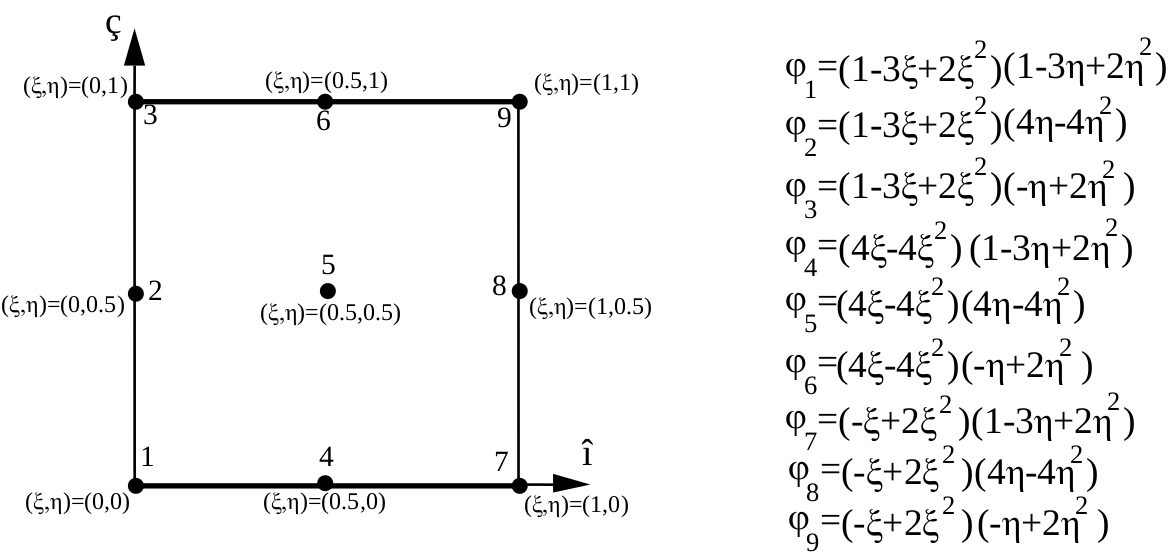
\includegraphics[scale=0.3]{biquadratic.png}
\caption{The shape functions on the 9-node reference element}\label{Figure1}
\end{center}
\end{figure*}

\newpage
\subsection{The semi-discrete approximation}
The discrete in space counterpart of (18),(19) reads:\\


Find $\mu_h, \phi_h \in V_h$ such that the equations hold for all $t \in (0, T]$.

\begin{align}
\int_\Omega \mu_h\eta \, dx -\int_\Omega \nabla\phi_h\cdot \nabla\eta \, dx - \frac{1}{\epsilon^2}\int_\Omega  W'(\phi_h)\eta
&= 0  \:\:\:\:\:\:\:\: ,\forall \eta \in V_h \\
\int_\Omega\frac{\partial \phi_h}{\partial t} \psi \, dx + \gamma\int_\Omega \nabla \mu_h \cdot \nabla \psi \, dx &= 0 
 \:\:\:\:\:\:\:\: ,\forall \psi \in V_h
\end{align}



Next, to compute the finite element approximation $\mu_h$ and $\phi_h$, we let $\{\psi_i\}_{i=1}^N$ be the quadratic Lagrange polynomial functions for the subspace $V_h$. We project $\mu$ and $\phi$ to $V_h$, so that they can be written as:

\begin{align}
\mu_h(t) &= \sum_{j=1}^N \mu_j(t) \psi_j \\
\phi_h(t) &= \sum_{j=1}^N \phi_j(t) \psi_j
\end{align}

with $2N$ time-dependent unknowns $\mu_j(t)$, $\phi_j(t)$ for $j = 1, 2, \ldots, N$ to be found.\\


Inserting (22),(23) to (21),(22) and using the quadratic test functions for $\eta,\psi$ in the relations above, we obtain:

\begin{align}
\int_\Omega \sum_{j=1}^N \mu_j(t) \psi_j\psi_i \, dx -\int_\Omega \nabla(\sum_{j=1}^N \phi_j(t) \psi_j)\cdot \nabla\psi_i \, dx - \frac{1}{\epsilon^2}\int_\Omega  W'(\sum_{j=1}^N \phi_j(t) \psi_j)\psi_i
&= 0\\ 
\int_\Omega\frac{\partial \sum_{j=1}^N \phi_j(t) \psi_j}{\partial t} \psi_i \, dx + \gamma\int_\Omega \nabla (\sum_{j=1}^N \mu_j(t) \psi_j) \cdot \nabla \psi_i \, dx &= 0 
\end{align} \\\\\\


\subsection{The fully dicrete problem}
Using the fact that the nodal coefficients $\mu_j(t)$, $\phi_j(t)$ for $j = 1, 2, \ldots, N$ are only of temporal dependence and since we can interchange the (finite) summation with the integral, we can deduce the form of the mass, stiffness matrices and of the non linear term respectively, that correspond to the fully discrete version of the problem. These are:\\

\begin{align}
M_{ij} &= \int_{\Omega} \psi_i\psi_j \, dx, \quad for \quad i, j = 1, 2, \ldots, N \\
A_{ij} &= \int_{\Omega} \nabla \psi_i\cdot\nabla \psi_j \, dx, \quad for \quad i, j = 1, 2, \ldots, N \\
W'(\phi(t))_{ij} &= \int_\Omega  W'(\sum_{j=1}^N \phi_j(t) \psi_j)\psi_i,\quad for \quad j = 1, 2, \ldots, N
\end{align}\\


Spatial discretization in vector-matrix notation reads as follows:\\

Find  $\mu_j(t)$, $\phi_j(t)$ for $j = 1, 2, \ldots, N$ such that:\\

\begin{align}
M\vec{\mu}(t) - A\vec{\phi}(t)- \frac{1}{\epsilon^2}W'(\vec{\phi}(t)) &= 0 \\
M\frac{\partial \vec{\phi}(t)}{\partial t} + \gamma A\vec{\mu}(t) &= 0 
\end{align}\\

where $t \in (0, T].$

\section{The temporal discretization}
This chapter is of general significance as it serves as a general outline for the available time schemes that can be applied to phase field models and presents some of the critical subtleties concerning the characteristic parameters of the modelling. Here we follow \cite{inbook}.
In the consideration of time-discrete schemes , we are concerned with the following properties:
\begin{enumerate}
    \item the order of accuracy of the scheme,
    \item the stability of the algorithm,
    \item the solvability of the time-discrete equations.
\end{enumerate}

In the context of linear problems, stability is associated with the decay of the time-discrete solution with time, a feature also attained by the exact solution of stable linear problems. When the stability of the time discrete solution is achieved independently of $\tau$, the time-integration scheme is said to be unconditionally stable. If stability holds under some constraint (e.g., on the time-step size), then the scheme is said to be conditionally stable. Explicit time integration algorithms which are consistent are always conditionally stable, while implicit schemes might be unconditionally stable.

For nonlinear problems, the situation is more complicated than for linear equations due to the several notions of stability that may be defined for different problems and as unconditionally stable schemes is not identical to making the algorithm implicit. Because of the energetic structure behind phase-field models, natural notions of stability are those related to free-energy dissipation. In particular, a numerical scheme is said to be unconditionally energy- (or gradient-, or nonlinearly) stable if:
\begin{equation}
    E(\phi_{n+1}) - E(\phi_n) \leq 0 \quad \text{for all } n \geq 0. \label{eq:energy_stability}
\end{equation}

In the consideration of time-discrete schemes \cite{Hairer1987, Hughes2012},properties of significance are:
\begin{enumerate}
    \item the order of accuracy of the scheme,
    \item the stability of the algorithm,
    \item the solvability of the time-discrete equations.
\end{enumerate}


In other words, the scheme preserves the energy-dissipative property of the underlying model, in the sense that it dissipates energy at each time step. Analogously to the linear case, if (\ref{eq:energy_stability}) holds under some constraint, then the scheme is said to be conditionally energy stable.

In analyzing time-integration schemes for phase-field theories, one needs to be specific about the smoothness of the particular chosen double well function $W(\phi)$. Two common assumptions are:

\begin{itemize}
    \item $\mathbf{(A1)}$ $W \in C^0[a, b] \cap C^2(a, b)$ with $-\infty \leq a < b \leq \infty$, and $W''$ is bounded below, i.e., $W$ is continuous on the bounded interval $[a, b]$ and at least twice differentiable on the open interval $(a, b)$, and there is a constant $\kappa_W > 0$ such that
    \begin{equation}
        W''(\phi) \geq -\kappa_W \text{ for all } \phi \in (a, b).
    \end{equation}
    \item $\mathbf{(A2)}$ $W \in C^{2,1}(\mathbb{R})$, i.e., $W''$ is globally Lipschitz continuous. This means that there is a constant $L_W > 0$ such that
    \begin{equation}
        \left|W''(\phi)\right| \leq L_W \text{ for all } \phi \in \mathbb{R}.
    \end{equation}
\end{itemize}

Note that if $W$ satisfies $\mathbf{(A2)}$, then it also satisfies $\mathbf{(A1)}$ (with $a = -\infty$, $b = \infty$, and $\kappa_W = L_W$), but not vice versa. In particular, the classical quartic potential
\begin{equation}
    W(\phi) = \frac{1}{4}(1 - \phi^2)^2
\end{equation}
satisfies $\mathbf{(A1)}$ with $a = -\infty$ and $b = \infty$, but it does not satisfy $\mathbf{(A2)}$. The logarithmic potential
\begin{equation}
    W(\phi) = \frac{1}{2}\left((1 + \phi)\log\left(1 + \frac{\phi}{2}\right) + (1 - \phi)\log\left(1 - \frac{\phi}{2}\right) + \theta(1 - \phi^2)\right)
\end{equation}
satisfies $\mathbf{(A1)}$ with $a = -1$ and $b = 1$, and it also does not satisfy $\mathbf{(A2)}$. On the other hand, the truncated quartic potential
\begin{equation}
    W(\phi) = \begin{cases}
        (\phi + 1)^2 & \text{if } \phi < -1 \\
        \frac{1}{4}(1 - \phi^2)^2 & \text{if } \phi \in [-1, 1] \\
        (\phi - 1)^2 & \text{if } \phi > 1
    \end{cases}
\end{equation}
 satisfy  $\mathbf{(A1)}$ (with $a = -\infty$ and $b = \infty$) and $\mathbf{(A2)}$.

\subsection{First-order accurate schemes}

We now consider first-order schemes for the Cahn--Hilliard equation. All of the schemes are implicit in some sense, since explicit schemes for fourth-order parabolic problems are infeasible.

\subsubsection{Backward Euler}

The backward Euler method applied to the Cahn--Hilliard equation leads to the system:
\begin{align}
    \frac{\phi_{n+1} - \phi_n}{\tau} &= \Delta \mu_{n+1} \\
    \mu_{n+1} &= W'(\phi_{n+1}) - \epsilon^2 \Delta \phi_{n+1}
\end{align}

This method is nonlinearly implicit because it requires the solution of a nonlinear system for the pair $(\phi_{n+1}, \mu_{n+1})$. Implicit schemes which are unconditionally linearly stable, such as the Backward Euler method, are generally conditionally stable for nonlinear problems. To see this, consider the energy difference:
\begin{equation}
    E(\phi_{n+1}) - E(\phi_n) = \int_{\Omega} \left(W(\phi_{n+1}) - W(\phi_n) + \frac{1}{2} \epsilon^2 |\nabla \phi_{n+1}|^2 - \frac{1}{2} \epsilon^2 |\nabla \phi_n|^2\right) \, dx
\end{equation}

Given two real numbers $u$ and $v$ that enclose $\xi$, we can use a Taylor's series expansion to show that:
\begin{equation}
    W(u) - W(v) - W'(u)(u - v) = -\frac{1}{2} W''(\xi)(u - v)^2 \leq \kappa_W \frac{(u - v)^2}{2}
\end{equation}

where the inequality holds due to assumption $\mathbf{(A1)}$, which is valid for all the potentials $W$ of interest. One then obtains:
\begin{equation}
    E(\phi_{n+1}) - E(\phi_n) \leq \int_{\Omega} \left(\mu_{n+1}(\phi_{n+1} - \phi_n) - \epsilon^2 \nabla \phi_{n+1} \cdot \nabla(\phi_{n+1} - \phi_n) + \kappa_W \frac{1}{2} (\phi_{n+1} - \phi_n)^2\right) \, dx
\end{equation}

Next, we bound $\|\phi_{n+1} - \phi_n\|_2^2$ using the equation for $\phi_{n+1}$:
\begin{align}
    \int_{\Omega} (\phi_{n+1} - \phi_n)^2 \, dx &= -\tau \int_{\Omega} \nabla \mu_{n+1} \cdot \nabla(\phi_{n+1} - \phi_n) \, dx \\
    &\leq \tau \frac{1}{2\delta} \int_{\Omega} |\nabla \mu_{n+1}|^2 \, dx + \tau \delta \int_{\Omega} |\nabla(\phi_{n+1} - \phi_n)|^2 \, dx
\end{align}

where the last inequality holds for any $\delta > 0$. Finally, choosing $\delta = \frac{2\epsilon^2}{\kappa_W\tau}$ gives:
\begin{equation}
    E(\phi_{n+1}) - E(\phi_n) \leq -\tau \left(1 - \frac{\kappa_W^2\tau\epsilon^2}{8}\right) \int_{\Omega} |\nabla \mu_{n+1}|^2 \, dx
\end{equation}

Therefore, if:
\begin{equation}
    \tau < \frac{8\epsilon^2}{\kappa_W^2}
\end{equation}

then (\ref{eq:energy_stability}) holds. In other words, the backward Euler scheme is conditionally energy stable.
Furthermore, it can be shown that under the same time-step constraint, the nonlinear system (38)--(39) has a unique solution for $(\phi_{n+1}, \mu_{n+1})$ if condition (46) holds. The proof of this can be found in, for example, \cite{Elliott1989}, and the underlying concept of the proof is applicable to other schemes.

To prove the existence of a solution, one demonstrates that the system represents the necessary condition (Euler-Lagrange equation) corresponding to a minimization problem for a convex functional. Subsequently, to prove the uniqueness of a solution, one follows similar steps to those used in establishing the energy stability mentioned earlier. It's worth noting that, since $\epsilon$ is generally very small, condition (46) imposes a severe constraint on the allowed time-step size.
\subsubsection{First-order semi-implicit method}
A popular scheme (Provatas and Elder, 2010) is the following first-order semi-implicit (or implicit/explicit) method:

\begin{equation}
\phi_{n+1} - \phi_n \tau = \Delta \mu_{n+1} \label{eq:203}
\end{equation}

\begin{equation}
\mu_{n+1} = W'(\phi_n) - \epsilon^2 \Delta \phi_{n+1} \label{eq:204}
\end{equation}

Because it treats $W'$ explicitly, it is a linear (or linearly-implicit) method requiring the solution of a linear system at each time step. The system can be written abstractly as:

\begin{equation}
\begin{bmatrix}
\mu_{n+1} \\
\phi_{n+1}
\end{bmatrix}
=
\begin{bmatrix}
\phi_n \\
-W'(\phi_n)
\end{bmatrix} \label{eq:205}
\end{equation}

where $B$ is the differential operator defined by:

\begin{equation}
B =
\begin{bmatrix}
-\tau \Delta & -I \\
-I & -\epsilon^2\Delta
\end{bmatrix} \label{eq:206}
\end{equation}

Here, $I$ denotes the identity operator. The linear system of differential equations (\ref{eq:205}) has a unique solution, independent of $\tau$. This follows from the coercivity estimate:

\begin{equation}
\int_{\Omega}
\begin{bmatrix}
\mu_{n+1} \\
\phi_{n+1}
\end{bmatrix}
\cdot B
\begin{bmatrix}
\mu_{n+1} \\
\phi_{n+1}
\end{bmatrix}
dx = \tau \|\nabla\mu_{n+1}\|^2 + \epsilon^2\|\nabla\phi_{n+1}\|^2 \label{eq:207}
\end{equation}

as well as mass conservation $\int_{\Omega}(\phi_{n+1} - \phi_n)dx = 0$ and the condition $\int_{\Omega} \mu_{n+1} dx = \int_{\Omega} W'(\phi_n) dx$.

However, as may be expected, the method is only conditionally energy stable. In fact, we can only show conditional stability if $W$ satisfies $(A2)$. Let us assume that $\xi$ is an undetermined point of the interval $(0, 1)$. Then,

\begin{equation}
E(\phi_{n+1}) - E(\phi_n) = -\tau \|\nabla\mu_{n+1}\|^2 + \frac{1}{2} \int_{\Omega} W''(\phi_{n+\xi})(\phi_{n+1} - \phi_n)^2dx - \frac{1}{2}\epsilon^2\|\nabla(\phi_{n+1} - \phi_n)\|^2 \label{eq:208}
\end{equation}
\begin{equation}
\leq -\tau \|\nabla\mu_{n+1}\|^2 + \frac{LW^2}{2} \|\phi_{n+1} - \phi_n\|^2 - \frac{\epsilon^2}{2} \|\nabla(\phi_{n+1} - \phi_n)\|^2 \label{eq:208}
\end{equation}

where $\phi_{n+\xi} \approx \phi(\cdot, t_n + \xi\tau)$. The inequality (\ref{eq:208}) is identical to (200) replacing $\kappa W$ with $LW$. Therefore, following the same steps as in Sect. 4.1.1, leads to the similar constraint $\tau < \frac{8\epsilon^2}{L^2W}$ for energy stability.
\subsubsection{Convex-Splitting Method}

The stability issues for the backward Euler and semi-implicit methods originate from the nonconvexity of $W(\phi)$. A groundbreaking idea, which goes back to \cite{Elliott1993TheGD} and was popularized by \cite{Eyre1998UnconditionallyGS}, is to split $W$ into a convex part and a concave part, i.e.,

\begin{equation}
W(\phi) = W_{+}(\phi) + W_{-}(\phi)
\end{equation}

with $W''_{+}(\phi) \geq 0$ and $W''_{-}(\phi) \leq 0$ \cite{cite_key}. Then, we treat $W_{+}$ implicitly and $W_{-}$ explicitly, as

\begin{equation}
\phi_{n+1} - \phi_n = \frac{\Delta \mu_{n+1}}{\tau}
\end{equation}

\begin{equation}
\mu_{n+1} = W'_{+}(\phi_{n+1}) + W'_{-}(\phi_n) - \frac{\epsilon^2}{2}\Delta\phi_{n+1}
\end{equation}


Using Taylor's formulas, we have

\begin{equation}
W_{+}(\phi_{n+1}) = W_{+}(\phi_n) + W_{+}'(\phi_{n+1})(\phi_{n+1} - \phi_n) - \frac{1}{2}W_{+}''(\phi_{n+\xi})(\phi_{n+1} - \phi_n)^2
\end{equation}

\begin{equation}
W^-(\phi_{n+1}) = W^-(\phi_n) + W^-(\phi_n)(\phi_{n+1} - \phi_n) + \frac{1}{2} W''^-(\phi_n + \zeta)(\phi_{n+1} - \phi_n)^2
\end{equation}

where $\xi, \zeta \in (0, 1)$. The energy difference is now

\begin{equation}
E(\phi_{n+1}) - E(\phi_n) = -\tau \|\nabla\mu_{n+1}\|^2 - \frac{1}{2}\int_\Omega \left(W''_{+}(\phi_{n+\xi}) - W''_{-}(\phi_{n+\zeta})\right)(\phi_{n+1} - \phi_n)^2 dx - \frac{1}{2}\epsilon^2\|\nabla(\phi_{n+1} - \phi_n)\|^2
\end{equation}

which shows the unconditional stability of the method. If $W$ satisfies (A1), then the above convex splitting is non-unique, but it is always possible. For instance, defining

\begin{equation}
W^-(\phi) = -\kappa W \frac{\phi^2}{2}
\end{equation}

and subsequently setting $W^+(\phi) = W(\phi) - W^-(\phi)$. Unique solvability of the system (210) follows by equivalence with a strictly-convex minimization problem. Hence, the convex-splitting scheme is both unconditionally stable and unconditionally solvable. If, in addition, (A2) applies, then a splitting is possible with $W^+(\phi)$ being a quadratic polynomial, i.e., defining

\begin{equation}
W^+(\phi) = L\frac{W}{2}\phi^2
\end{equation}

and subsequently setting $W^-(\phi) = W(\phi) - W^+(\phi)$. In this case, the scheme becomes even linear. 



\subsection{Stability and Solvability Analysis for Second-order Schemes}

\subsubsection{Crank–Nicolson Method}
The Crank–Nicolson method is defined as follows:
\begin{align}
    \frac{\phi_{n+1} - \phi_n}{\tau} &= \frac{\Delta \mu_{n+1}}{2} \label{eq:cn_phi} \\
    \frac{\mu_{n+1}}{2} &= \frac{W'(\phi_{n+1}) + W'(\phi_n)}{2} - \frac{\epsilon^2\Delta \phi_{n+1} + \phi_n}{2} \label{eq:cn_mu}
\end{align}

It requires the solution of a nonlinear system at each time step. Using the trapezoidal quadrature rule, we have
\begin{equation}
    W(v) - W(u) = \int_{u}^{v} W'(s) \, ds = W'(u) + W'(v) - \frac{1}{12}W'''(\xi)(v - u)^3 \label{eq:cn_trapezoidal}
\end{equation}

where $\xi$ is an unknown point that lies between $u$ and $v$. Then, it can be shown that the energy difference is given by:
\begin{equation}
    E(\phi_{n+1}) - E(\phi_n) = -\tau\|\nabla \mu_{n+1}\|^2 - \frac{1}{12}\int_{\Omega} W'''(\xi)(\phi_{n+1} - \phi_n)^3 \, dx \label{eq:cn_energy_difference}
\end{equation}

The sign of the last term in \eqref{eq:cn_energy_difference} cannot be controlled, making the method generally not unconditionally energy stable. Furthermore, the solvability of this method, corresponding to a nonconvex nonlinear system, also suffers from a time-step constraint, $\tau \leq C\epsilon^2/\kappa_W^2$, similar to the backward Euler scheme.

\subsubsection{Second-order Semi-implicit Method}
The second-order semi-implicit method is defined as:
\begin{align}
    \frac{\phi_{n+1} - \phi_n}{\tau} &= \frac{\Delta \mu_{n+1}}{2} \label{eq:second_order_semi_implicit_phi} \\
    \frac{\mu_{n+1}}{2} &= W'(\phi_n) + \frac{1}{2}W''(\phi_n)(\phi_{n+1} - \phi_n) - \frac{\epsilon^2\Delta \phi_{n+1} + \phi_n}{2} \label{eq:second_order_semi_implicit_mu}
\end{align}

This method is linear and corresponds to the following system:
\begin{equation}
    \begin{bmatrix}
    \mu_{n+1} \\
    \phi_{n+1}
    \end{bmatrix}
    =
    \begin{bmatrix}
    \phi_n - W'(\phi_n) + \frac{1}{2}W''(\phi_n)\phi_{n+1} - \frac{1}{2}\epsilon^2\Delta\phi_{n+1} \\
    \phi_n
    \end{bmatrix}
\end{equation}

The linear system of differential equations for this method has a unique solution, independent of $\tau$. This follows from the coercivity estimate, as well as mass conservation and the condition $\int_\Omega \mu_{n+1} \, dx = \int_\Omega W'(\phi_n) \, dx$. However, this method is conditionally energy stable, and the condition $\tau < 8\epsilon^2/L_W^2$ is needed for unconditional energy stability.

\subsubsection{Secant Method}
The secant method, designed to mimic the energy dissipation, is defined as:
\begin{align}
    \frac{\phi_{n+1} - \phi_n}{\tau} &= \frac{\Delta \mu_{n+1}}{2} \label{eq:secant_phi} \\
    \frac{\mu_{n+1}}{2} &= DW(\phi_n, \phi_{n+1}) - \frac{\epsilon^2\Delta \phi_{n+1} + \phi_n}{2} \label{eq:secant_mu}
\end{align}

Here, $DW(\phi, \psi)$ is the discrete variational derivative defined as:
\begin{equation}
    DW(\phi, \psi) = \int_0^1 W'(\phi + s(\psi - \phi)) \, ds
\end{equation}
Alternatively, the discrete variational derivative can be expressed as:

\begin{equation}
DW(\phi_n, \phi_{n+1}) = \begin{cases}
\frac{W(\phi_{n+1}) - W(\phi_n)}{\phi_{n+1} - \phi_n} & \text{if } \phi_{n+1} \neq \phi_n \\
W'(\phi_n) & \text{if } \phi_{n+1} = \phi_n
\end{cases}
\end{equation}

This formulation explains the name of the method. By observing that

\begin{equation}
DW(\phi_n, \phi_{n+1})(\phi_{n+1} - \phi_n) = W(\phi_{n+1}) - W(\phi_n)
\end{equation}

it can be deduced that the method is unconditionally energy stable, as indicated by the relation

\begin{equation}
E(\phi_{n+1}) - E(\phi_n) = -\tau \|\nabla \mu_{n+1}\|^2.
\end{equation}

However, due to the non-convex nature of \(W\), the nonlinear system (69)–(70) is only conditionally solvable (Elliott, 1989). The operator \(DW\)  finds extensive use in the development of exact energy-preserving schemes. This method is unconditionally energy stable, but the solvability of the nonlinear system \eqref{eq:secant_phi}--\eqref{eq:secant_mu} is conditional.
Several variants that avoid constructing the secant while maintaining stability are as follows:

1. Implicit Taylor Method:
\begin{align}
DW(\phi_n, \phi_{n+1}) &= W'(\phi_{n+1}) - \frac{1}{2}W''(\phi_{n+1})(\phi_{n+1} - \phi_n) \notag\\
&\qquad + \frac{1}{3!}W'''(\phi_{n+1})(\phi_{n+1} - \phi_n)^2 \tag{75}
\end{align}

2. Method by Gomez and Hughes (2011):
\begin{equation}
DW(\phi_n, \phi_{n+1}) = \frac{1}{2}\left(W'(\phi_n) + W'(\phi_{n+1})\right) - \frac{1}{12}W'''(\phi_n)(\phi_{n+1} - \phi_n)^2 \tag{76}
\end{equation}

These methods lead to the following energy change:
\begin{equation}
E(\phi_{n+1}) - E(\phi_n) = -\tau \|\nabla \mu_{n+1}\|^2 - \frac{1}{24}\int_{\Omega}W''''(\phi_{n+\xi})(\phi_{n+1} - \phi_n)^4 \; d\Omega, \; \xi \in (0, 1) \tag{77}
\end{equation}

The last term is negative or zero if \(W'''' \geq 0\). This inequality holds for all potential functions. If the potential \(W\) does not satisfy the condition \(W'''' \geq 0\), Gomez and Hughes (2011) propose a splitting of \(W\) that achieves second-order accuracy and unconditional stability.
Considering that the methods described in this section correspond to non-convex nonlinear systems, their solvability is conditional.

\subsubsection{Second-order Convex Splitting} 

In an effort to achieve both unconditional stability and solvability, a second-order time-accurate convex-splitting scheme was proposed by Hu et al. (2009). The method is described by the following equations:

\begin{align}
\phi_{n+1} - \phi_n &= \frac{1}{2}\Delta\mu_{n+1} \tag{234} \\
\mu_{n+1}^{2} &= DW_{+}(\phi_{n+1}, \phi_n) + DW_{-}(\phi_n, \phi_{n-1}) - \frac{\varepsilon^2}{2}\Delta\phi_{n+1} + \frac{\phi_{n+1} + \phi_n}{2} \tag{78}
\end{align}

Where:
- \(DW_{+}(\phi_{n+1}, \phi_n)\) is defined as:
\begin{equation}
DW_{+}(\phi_{n+1}, \phi_n) = \int_{0}^{1} W'(\phi_n + s(\phi_{n+1} - \phi_n)) \, ds \tag{79}
\end{equation}
- \(DW_{-}(\phi_n, \phi_{n-1})\) is defined as:
\begin{equation}
DW_{-}(\phi_n, \phi_{n-1}) = \frac{3}{2}W'_{-}(\phi_n) - \frac{1}{2}W'_{-}(\phi_{n-1}) \tag{80}
\end{equation}

This method employs a secant treatment of the convex part and a two-step second-order backward difference treatment of the concave part. While this method is unconditionally solvable, it does not meet the criteria for unconditional stability. A less restrictive condition, referred to as weak energy stability (Hu et al., 2009), may be established if \(W_{-}\) is a quadratic polynomial, which holds for many potential functions. An alternative approach is the multistep scheme proposed in (Guillén-González and Tierra, 2013), which, however, is limited to quartic potentials. This alternative scheme is linear, unconditionally energy stable (with a modified energy statement), and unconditionally uniquely solvable. The above and the following references can be found in the main \cite{inbook}
\subsection{Stabilization}
Most second-order linear schemes suffer from conditional stability and/or conditional solvability. As proposed by Wu et al. (2014), these issues can be stabilized if $W$ satisfies (A2). For example, the stabilized semi-implicit scheme is given as follows:

\begin{align}
\phi_{n+1} - \phi_n &= \frac{\Delta\mu_{n+1}}{2} \tag{81} \\
\mu_{n+1}^{2} &= W'(\phi_n) + \frac{1}{2}W''(\phi_n)(\phi_{n+1} - \phi_n) - \frac{\varepsilon^2}{2}\Delta\phi_{n+1} + \frac{\phi_{n+1} + \phi_n}{2} - \beta\tau\Delta(\phi_{n+1} - \phi_n) \tag{82}
\end{align}

Here, $\beta$ is the stabilization parameter. Such terms are also referred to as artificial viscosity and are useful in many applications (see, e.g., Labovsky et al., 2009; Jansen et al., 2000). For a stabilization of the extended Crank–Nicolson method, refer to Gomez and Hughes (2011).

Using Taylor's formula, it can be shown that:

\begin{equation}
\begin{aligned}
E(\phi_{n+1}) - E(\phi_n) &= -\tau \|\nabla\mu_{n+1}\|^2 + \frac{1}{2}\int_{\Omega}\left(W''(\xi) - W''(\phi_n)\right)(\phi_{n+1} - \phi_n)^2\,d\Omega \\
&\quad - \beta\tau\|\nabla(\phi_{n+1} - \phi_n)\|^2 
\end{aligned}
\end{equation}

Then, assuming that $W$ satisfies (A2):

\begin{equation}
\begin{aligned}
E(\phi_{n+1}) - E(\phi_n) &\geq -\tau \|\nabla\mu_{n+1}\|^2 + L W\|\phi_{n+1} - \phi_n\|^2 \\
&\quad - \beta\tau\|\nabla(\phi_{n+1} - \phi_n)\|^2  \\
&\geq -\tau\left(1 - \frac{LW}{2\delta}\right)\|\nabla\mu\|^2 - \tau\left(\beta - \frac{LW}{\delta}\right)\|\nabla(\phi_{n+1} - \phi_n)\|^2 \text{ (by Young's inequality with } 0 < \delta < \frac{LW}{2}\text{)}.
\end{aligned}
\end{equation}

Therefore, for $\beta > \frac{L^2_W}{4}$, one has unconditional energy stability. It is worth noting that unconditional solvability follows by mimicking the proof for the Backward Euler method, as described in the work of Elliott \cite{Elliott1989}.




\section{The Newton-Raphson procedure}


In this section, we briefly discuss the simplest multidimensional root finding
method, the Newton-Raphson method. This method provides an efficient means of
converging to a root when a sufficiently good initial data is given but, when this is not feasible it can fail to converge, indicating, though not proving, that a nearby root does not exist. For our implementation the initial guess has to be the combined solution of the previous time step, which for the most cases will work well. For the contained description we do not pose the following thoughts with a mathematical rigor but rather with the more intuitive approach.\\

We consider $N$ functional relations that need to be set to zero and are represented as:

\[
F_i(x_1, x_2, \ldots, x_N) = 0, \quad i = 1, 2, \ldots, N. \label{eq:functional_relations}
\]


In the neighborhood of vector $x$, each function $F_i$ can be expanded using a Taylor series:

\[
F_i(x + \delta x) = F_i(x) + \sum_{j=1}^{N} \frac{\partial F_i}{\partial x_j} \delta x_j + O(\delta x^2). \label{eq:taylor_series}
\]

The matrix $J$ of partial derivatives appearing in the previous equation is the Jacobian matrix, with entries:

\[
J_{ij} \equiv \frac{\partial F_i}{\partial x_j}. \label{eq:jacobian_matrix}
\]

In matrix notation we have:

\[
\mathbf{F}(\mathbf{x} + \delta \mathbf{x}) = \mathbf{F}(\mathbf{x}) + J \delta \mathbf{x}. \label{eq:matrix_notation}
\]

By neglecting terms of order $\delta x^2$ and setting $\mathbf{F}(\mathbf{x} + \delta \mathbf{x}) = 0$, we obtain a set of linear equations for the corrections $\delta \mathbf{x}$ that simultaneously move each function closer to zero:

\[
J \cdot \delta \mathbf{x} = -\mathbf{F}. \label{eq:linear_equations}
\]

The matrix equation is then solved and the corrections are then added to the solution vector:

\[
\mathbf{x}_{\text{new}} = \mathbf{x}_{\text{old}} + \delta \mathbf{x}. \label{eq:solution_update}
\]

The process is iterated until convergence is achieved. In general, it is advisable to check the degree to which both functions and variables have converged. Once either reaches machine accuracy, the other is unlikely to change. In our problem the presence of the double well potential accounts for the non-linearity of the Cahn-Hilliard model and of the arising discrete system of algebraic equations. Using a Taylor's expansion of the vector field of equations around the combined solution vector we achieve a linear approximation of the system. At each (fixed) time step $t_n$, we employ this iterative algorithm to solve it.\\
 Let us consider that a standard backward Euler scheme is applied and let $S_n = (\vec{\mu}_n, \vec{\phi}_n)$ denote the combined vector of unknowns. We state the relations (32),(33) as:
\begin{equation}
F^n_{vec}(S_n) = 0.
\end{equation}
where the residual $F^n_{vec}$ is defined by:
\begin{align}
F^n_{vec}(S_n)_i = M \vec{\mu}_n - A \vec{\phi}_{n} - \frac{1}{\epsilon^2}f(\vec{\phi}_{n})\quad for\quad i = 1, 2, \ldots, N\\
F^n_{vec}(S_n)_i = M(\vec{\phi}_{n}-\vec{\phi}_{n-1})+ \gamma \Delta t A \vec{\mu}_n \quad for\quad i = N+1, \ldots, 2N
\end{align}

Assuming a reasonable initial guess $S_{n;0}$ of the solution $S_n = (\vec{\mu}_,n \vec{\phi}_n)$, we iteratively solve the linearized equation and update the solution vector as follows:
\begin{align}
J(S_{n;s})\Delta S_{n;s} = -F^n_{vec}(X_{n;s}), \\ 
S_{n;s+1} = S_{n;s} + \Delta S_{n;s}, \quad s = 0, 1, \ldots
\end{align}\\

where the entries of the Jacobian matrix $J$ are $J_{i,j}(S_n) = \frac{\partial F^n_{vec}{i}}{\partial S_nj}$, $i, j = 1, 2, \ldots, 2N$.\\


The iteration process is stopped below a certain tolerance (for instance, $||\Delta S_n||_{2} < \epsilon$).\\

For the calculation of the entries of the Jacobian matrix $J$, we differentiate the residual vector with respect to the nodal unknowns of the current timestep and we have:\\
\begin{align}
\frac{\partial (M \vec{\mu}_n - A \vec{\phi}_{n} - \frac{1}{\epsilon^2}W'(\vec{\phi}_{n}))}{\partial\vec{\mu_n}_j} &= M_{ij}, \\
\frac{\partial (M \vec{\mu}_n - A \vec{\phi}_{n} - \frac{1}{\epsilon^2}W'(\vec{\phi}_{n}))}{\partial\vec{\phi_n}_j} &= A_{ij}-\frac{1}{\epsilon^2}\frac{\partial W'(\vec{\phi_n})}{\partial \vec{\phi_n}_j}, \\
\frac{\partial (M(\vec{\phi}_{n}-\vec{\phi}_{n-1})+ \gamma \Delta t A \vec{\mu}_n)}{\partial\vec{\mu_n}_j} &= \gamma\Delta t A_{ij}, \\
\frac{\partial (M(\vec{\phi}_{n}-\vec{\phi}_{n-1})+ \gamma \Delta t A \vec{\mu}_k)}{\partial\vec{\phi_n}_j} &= M_{ij} 
\end{align}
where $M_{ij}$, $A_{ij}$, represent the entries of the mass and stiffness matrices $M$, $A$, respectively.\\

For the derivative of the non-linear term $W'(\vec{\phi_n})$, the dependence on the solution forces us to employ the chain rule:\\

\begin{equation}
\frac{\partial W'(\phi_n)_i}{\partial \phi_{nj}} = \frac{\partial W'}{\partial \phi_{n}} \frac{\partial \phi_n}{\partial{\phi_n}_j}= ((3(\sum_{l=1}^N\phi_{l}\psi_{l})^2-1)\psi_{i},\psi_{j})
\end{equation}


Provided that the Jacobian is invertible and $S_n$ is sufficiently close to the exact solution $S^*$, the procedure usually converges rapidly, namely, it holds:
\begin{equation}
||S_{n+1} - X^*|| \leq L ||S_n - S^*||^2
\end{equation}\\

\section{The algorithm for the Neumann case}
A contained description of the steps followed to solve the Neumann problem illustrate the core ideas of the implementation that can be adapted to the rest of the problems that we will examine, so it is proper to state them here:\\

1. Generate a spatial discretization for the rectangle $\Omega$ into 9-node elements and define the corresponding space of biquadratic polynomial functions $V_h$. Let $\psi_i$ for $i = 1, \ldots, N$ be the basis function for the subspace $V_h$.\\\\

2. Assemble the $N \times N$ mass matrix $M$ and the $N \times N$ stiffness matrix $A$ with entries:

\[
M_{ij} = \int_{\Omega} \psi_i \psi_j \, dx; \quad A_{ij} = \int_{\Omega} \nabla \psi_j \cdot \nabla \psi_i \, dx
\]\\\\

3. Create a time grid $0 = t_0 < t_1 < t_2 < \ldots < t_{n_{max}} = T$ on $0 < t < T$ with time steps $\Delta t_n = t_n - t_{n-1}$ for $n = 1, 2, \ldots, n_{max}$.\\\\

4. Choose initial condition $\mu_0$ and $\phi_0$. For this, either a random uniform sample is chosen from $[-1,1]$ and then we employ the Box-Muller transform to generate a desired normal initial distribution with given mean and variance, or an other choice is directly made.\\\\

5. Start the time point loop. For $n = 1, 2, \ldots, Tmax=n_{max}dt$ do:\\\\

6. Choose the starting guess $S_{n;0} = (\mu_{n-1}, \phi_{n-1})$ and a desired tolerance value $tol$ for the Newton-Raphson process.\\\\

7. Start the iterative process. For $iter = 1, 2, \ldots, iter_{max}$ do:\\\\

8. Assemble the nonlinear term $W'(\phi)$, the $N \times N$ Jacobian matrix $J$ of the nonlinear term and the $2N \times 1$ right-hand side of the Newton equation $-F^n_{vec}$, as shown in (35),(36). with entries:

\[
\begin{aligned}
W'({\phi}^{n,q})_i &= \int_{\Omega} ((\sum_{l=1}^N\phi_{l}\psi_{l})^3 - \sum_{l=1}^N\phi_{l}\psi_{l}) \psi_i \,dx, \quad l,i = 1, 2, \ldots, N \\
J_{ij}^{n,q} &= \int_{\Omega} ((3(\sum_{l=1}^N\phi_{l}\psi_{l})^2-1)\psi_{i},\psi_{j})dx, \quad l = 1, 2, \ldots, N \\    
\end{aligned}
\] \\\\ 

9. Assemble the global system matrix for the stationary system:\\
\begin{equation}
 F_{jac} = \left[ 
    \begin{array}{cc} 
      M & -J-\varepsilon^2A \\ 
      \Delta t A & M
    \end{array} 
    \right]
\end{equation}\\\\

10. Solve with the biconjugate gradient method (BiCGStab) the system:\\
\begin{equation}
F_{jac}\cdot \Delta S_{n,iter} = - F_{vec}
\end{equation}\\\\

11. Update the solution guess:\\
\begin{equation}
S_{n,iter+1} = S_{n,iter} + \Delta S_{n,iter}
\end{equation}\\\\

12. If the norm is below the tolerance value stop.\begin{equation}
||\Delta S_{n,iter}||_2 \quad < \quad tol
\end{equation} \\\\

13. End the Newton-iteration loop.\\\\

14. Set the solution vectors $\vec{\mu}_n$ and $\vec{\phi}_n$, with entries $\mu_{n_i} = {S_{n,iter}}_{i=1}^N$ and $\phi_{n_i} = {S_{n,iter}}_{N+1}^{2N}$.\\\\


15. End the time step loop in $n$.

\subsection{Results}
In this section we firstly consider the evolution of a random initial state $\phi_{0}=2r-1$, with $r$ following a uniform distribution on $[0,1]$. Here we consider a constant mobility set to $1$, the value of $\epsilon$ is $6.25\times10^{-2}$ and we opt for a constant $dt=5\times10^{-6}$ for the time of the simulation. The phase field evolution depicts the progressive formation and the coarsening of the two phases. The resolution is low due to the fine grid that was opted for low time-run purposes.
\clearpage
\vfill

\begin{figure}
\centering
\begin{subfigure}{.5\textwidth}
  \centering
  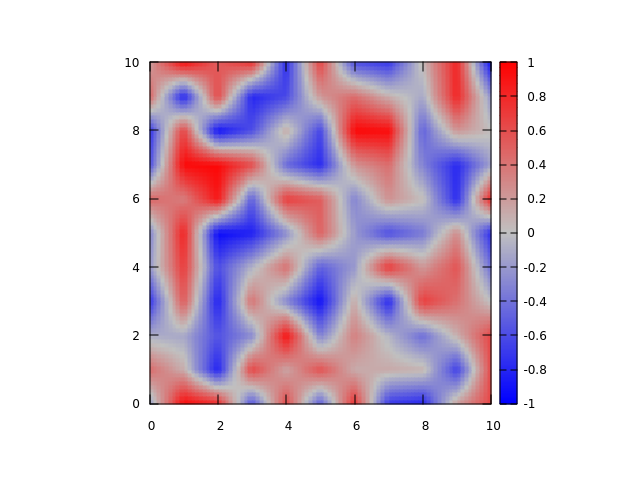
\includegraphics[width=1.0\linewidth]{initial.png}
  \caption{t=0}
  \label{fig:sub1}
\end{subfigure}%
\begin{subfigure}{.5\textwidth}
  \centering
  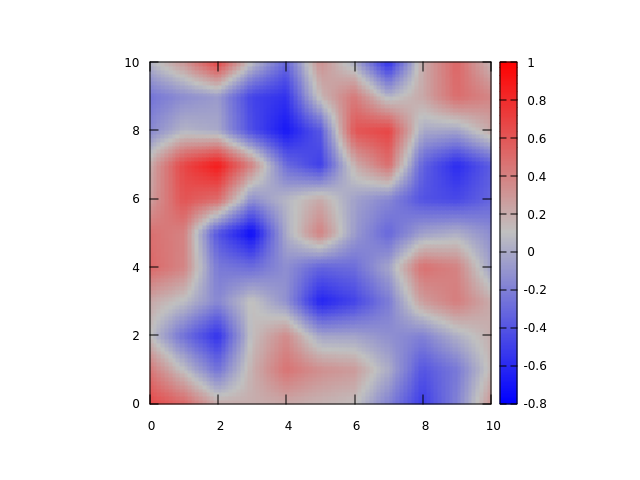
\includegraphics[width=1.0\linewidth]{100dt.png}
  \caption{t=100dt}
  \label{fig:sub2}
\end{subfigure}
\label{fig:test}
\end{figure}


\begin{figure}
\centering
\begin{subfigure}{.5\textwidth}
  \centering
  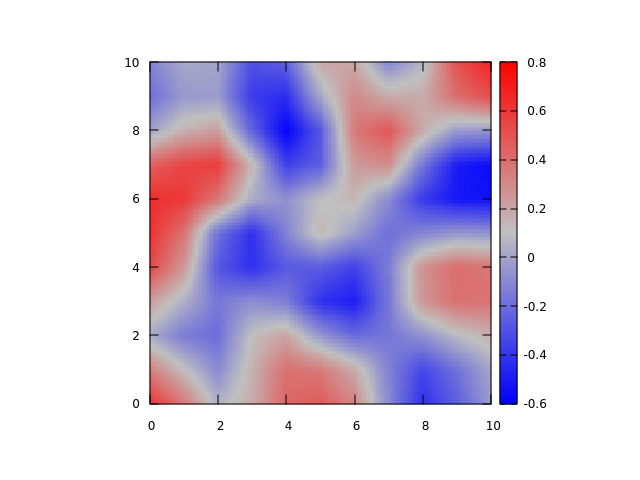
\includegraphics[width=1.0\linewidth]{500dt.png}
  \caption{t=500dt}
  \label{fig:sub1}
\end{subfigure}%
\begin{subfigure}{.5\textwidth}
  \centering
  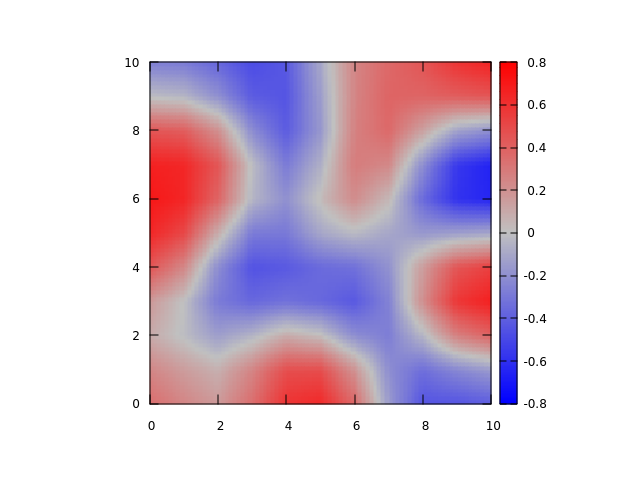
\includegraphics[width=1.0\linewidth]{2000dt.png}
  \caption{t=2000dt}
  \label{fig:sub2}
\end{subfigure}
\label{fig:test}
\end{figure}

\vfill
\begin{figure}
\centering
\begin{subfigure}{.5\textwidth}
  \centering
  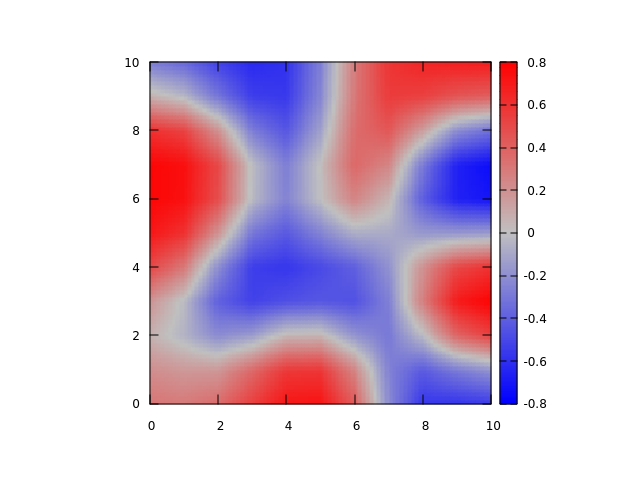
\includegraphics[width=1.0\linewidth]{3500dt.png}
  \caption{t=3500dt}
  \label{fig:sub1}
\end{subfigure}%
\begin{subfigure}{.5\textwidth}
  \centering
  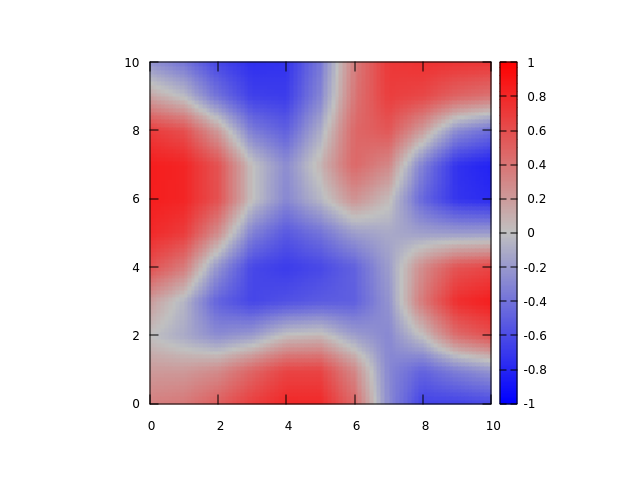
\includegraphics[width=1.0\linewidth]{5000dt.png}
  \caption{t=5000dt}
  \label{fig:sub2}
\end{subfigure}
\label{fig:test}
\end{figure}


\vfill
\clearpage


\section{The periodic problem}
 When considering periodic conditions in the context of the Cahn-Hilliard equation, it typically refers to solving this equation in a domain with periodic boundaries. This means that the material or system under investigation is assumed to exhibit periodic patterns of phase separation.This typically refers to a phenomenon in materials science or physics where two or more phases or components of a material segregate or separate from each other in a regular, repeating pattern. This can occur in various contexts, such as in materials with a periodic structure, under specific temperature and pressure conditions, or in the presence of external forces. 
        
\subsection{Statement of the problem}

For this chapter we will consider that the unit cell in $\Omega = \mathbb{R}^2$ is the characteristic domain of periodicity for our solution. Following (Elliott) we state the periodic problem for the Cahn-Hilliard equation as:\\

\begin{align}
\frac{\partial\phi}{\partial t} &= \gamma \nabla \cdot \left(\nabla \left(-\epsilon^2 \nabla^2 \phi +  W'(\phi)\right)\right) \text{ in } \Omega \times (0, T), \\
\frac{\partial^i \phi}{\partial x_j}|_{=0} &= \frac{\partial^i \phi}{\partial x_j}|_{=1}, \quad for\quad i=0,\dots 3\quad,\quad j=1,2 \text{ on } \overline{\Omega} \times (0, T), (C.M.Elliott-89) \\
\phi|_{t=0} &= \phi_0 \text{ in } \Omega
\end{align}\\


For this case we still consider the Ginzburg-Landau double well potential potential that was introduced in the first chapter:\\


\begin{equation}
W(\phi) = \frac{1}{4}(\phi^2 - 1)^2,
\end{equation}

with:

\begin{equation}
W'(\phi) = (\phi^2 - 1)\phi.
\end{equation}\\

Considering the problem set on a rectangle (or a unit square) the periodicity condition (50) forces the solution to attain the same values on opposite sides of the boundary:\\



\begin{align}
\phi(0,y,t) = \phi(1,y,t),\quad \forall y\in \overline{\Omega_y}\times(0,T]&\\
\phi(x,0,t) = \phi(x,1,t),\quad \forall x\in \overline{\Omega_x}\times(0,T]
\end{align}\\

These two relations will be used on the fully discrete scheme to impose explicitily the boundary conditions, as well as play a crucial role in the modifications that are needed for the general computational scheme proposed in the Neumann case to work. We follow the same steps to construct a mixed finite element form of the current problem.\\\\\\\\

\subsection{The weak formulation}

The difference in the integration against the standard test functions is that the boundary integral terms from the application of the second Green's identity does not vanish immediately, as in the zero flux case. For the simplified form we will technically procced to an approximation of the solution from a subspace that represents the boundary conditions.  The weak form becomes on the standard biquadratic functions becomes:

\begin{align}
\int_\Omega \mu\eta \, dx +\int_{\partial{\Omega}}\eta(\nabla\phi\cdot n)\,ds -\int_\Omega \nabla\phi\cdot \nabla\eta \, dx - \frac{1}{\epsilon^2}\int_\Omega  W'(\phi)\eta
&= 0\\
\int_\Omega\frac{\partial \phi}{\partial t} \psi \, dx -\int_{\partial{\Omega}}\psi(\nabla \mu\cdot n)\,ds + \gamma\int_\Omega \nabla \mu \cdot \nabla \psi \, dx &= 0
\end{align}\\
where $n$ denotes the surface normal vector.\\

\subsection{The finite dimensional projection of the solution}

Let $\{\psi_i\}_{i=1}^N$ be the biquadratic Lagrange polynomial functions, or any other choice, for the subspace $V_h$. Seeking approximations for $\mu$ and $\phi$ to $V_h$, so that they match at the nodal point with our functions we would once more begin with the following representations:\\

\begin{align}
\mu_{h}(t) &= \sum_{j=1}^N \mu_{j}(t) \psi_j \\
\phi_h(t) &= \sum_{j=1}^N \phi_j(t) \psi_j
\end{align}

with $2N$ time-dependent unknowns $\mu_j(t)$, $\phi_j(t)$ for $j = 1, 2, \ldots, N$ to be found.\\


At this point, the periodic setting of the problem, forces the same nodal values on the nodes of the opposing boundary sides, as we have identified the length of each dimension with the period length in the horizontal and the vertical directions.\\

For instance condition (50) leads to $\phi_{2} = \phi_{30},\quad \mu_{8} = \mu_{14}$ with the numbering of the nodes of Figure 2.

\begin{figure*}{b}
\begin{center}
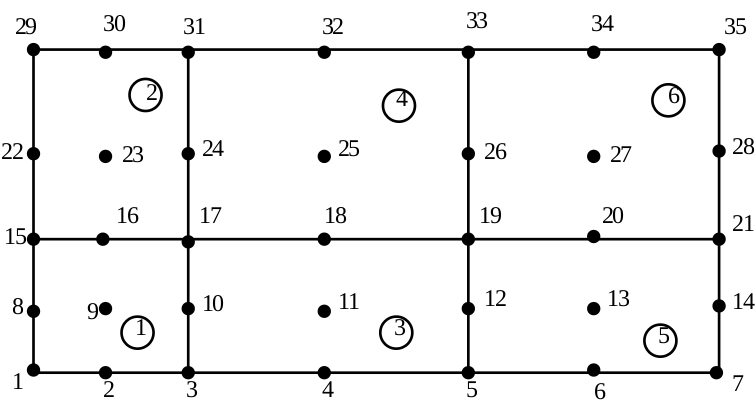
\includegraphics[scale=0.4]{rectangledomain2.png}
\caption{Domain discretization in 9-node elements}\label{Figure2}
\end{center}
\end{figure*}

For our global node numbering identification we shall now on opt for down to top and left to right scanning of the grid. Namely if we have $N_y$ nodes on ${x=0}$, $N_x$ nodes on ${y=0}$ the ascending order of the numbering is:\\
\begin{align}
N_{ij} = (j-1)N_{y} + i,\quad  j=1,\dots N_y\quad i=1,\dots N_x 
\end{align}\\

\begin{figure*}{b}
\begin{center}
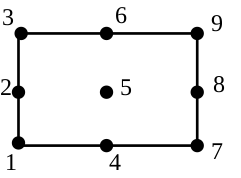
\includegraphics[scale=0.6]{numbering.png}
\caption{Down-top and Left-right numbering}\label{Figure3} 
\end{center}
\end{figure*}


For the $N_{max} = N = N_{x}N_{y}$ grid the periodic conditions mean:\\
\begin{align}
\phi_{i} = \phi_{N-N_{y}+i},\quad i =1,\dots,N_y\\
\phi_{(j-1)N_y+1} = \phi_{jN_{y}},\quad j =1,\dots,N_x
\end{align}\\
And the same relations hold for $\mu$ as a consequence of (50).\\

The practical significance is that we now operate on a smaller number of unkowns, namely: $ N-N_x-N_y$. The general representations shown above can now take a more specific form:

\begin{align}
\mu_h(t) &=  \sum_{j=1}^{N_y}\mu_{j}(\psi_{j}+\psi_{N-N_y+j}) + \sum_{i=1}^{N_x}\mu_{(i-1)N_y+1}(\psi_{(i-1)N_y+1}+\psi_{iN_y})+\sum_{inner}\mu_{j}\psi_{j}\\
\phi_h(t) &=  \sum_{j=1}^{N_y}\phi_{j}(\psi_{j}+\psi_{N-N_y+j}) + \sum_{i=1}^{N_x}\phi_{(i-1)N_y+1}(\psi_{(i-1)N_y+1}+\psi_{iN_y})+\sum_{inner}\phi_{j}\psi_{j}
\end{align}
The representations (64),(65) actually state that a different set of basis functions (and hence test functions since we are on Galerkin methods territory) is best fit for the periodic setting.\\
We denote the new basis and test functions as:\\

\begin{align}
\overline{\psi}_{j}&=(\psi_{j}+\psi_{N-N_y+j}),\quad j=1,\dots N_y,
\end{align}
\begin{align}
\overline{\psi}_{(i-1)N_y+1} &=(\psi_{(i-1)N_y+1}+\psi_{iN_y}),\quad   i=1,\dots N_x
\end{align}
\begin{align}
\overline{\psi}_{l}&=\psi_{l},\quad l\quad inner\quad node
\end{align}\\

\subsection{The system's matrices}
Based on the reduced (dimensionally) approximation of our functions, given by (64),(65), and following the same calculations of inserting those relations to the weak form of the problem, we calculate the necessary modifications of the matrices of the problem, to obtain the fully discrete scheme. To illustate these modifications, the mass matrix now becomes:

For $l$ inner node and $j$ left side node we have:

\begin{align}
\overline{M}_{lj} = \int_{\Omega} \overline{\psi}_l \overline{\psi}_j \, dx\\
= \int_{\Omega} \psi_l (\psi_{j}+\psi_{N-N_y+j}) \, dx \\
= \int_{\Omega} \psi_l \psi_j \, dx +\int_{\Omega} \psi_{l} \psi_{N-N_y+j} \, dx \\
= M_{lj} + M_{l;N-N_y+j} 
\end{align}\\

For $l$ inner node and $m=(i-1)N_y+1$ bottom side node we have:

\begin{align}
\overline{M}_{lm} = \int_{\Omega} \overline{\psi}_l \overline{\psi}_{(i-1)N_y+1} \, dx\\
= \int_{\Omega} \psi_l (\psi_{(i-1)N_y+1}+\psi_{iN_y}) \, dx \\
= \int_{\Omega} \psi_l \psi_{(i-1)N_y+1} \, dx +\int_{\Omega} \psi_{l} \psi_{iN_y} \, dx \\
= M_{l(i-1)N_y+1} + M_{l;iN_y} 
\end{align}\\

And the rest combinations follow in the same manner. These modifications apply also to the new stiffness matrix $\overline{A}$. Clearly the new matrices remain symmetric. The above modifications are inherited by the global system matrix presented in the previous chapter, as the mass, stiffness and the derivative matrix of the nonlinear term constitute the constructive blocks of the matrix.\\

\subsection{The nonlinear term}
For the handling of the nonlinear term:
\begin{align}
\overline{W'}({\phi})_i 
&= \int_{\Omega} ( \sum_{j=1}^{N_y}\phi_{j}\overline{\psi}_{j}+ \sum_{i=1}^{N_x}\phi_{(i-1)N_y+1}\overline{\psi}_{(i-1)N_y+1}+\sum_{inner}\phi_{j}\psi_{j})^3 - \sum_{j=2}^{N_y}\phi_{j}\overline{\psi}_{j}+ \sum_{i=2}^{N_x}\phi_{(i-1)N_y+1}\overline{\psi}_{(i-1)N_y+1}) \overline{\psi}_i+\sum_{inner}\phi_{j}\psi_{j} \,dx 
\end{align} \\\\




We need to notice that:\\

1. The inner product (integral) is linear in the second variable, so it can be split as a sum of integrals over the components of the new basis function $\overline{\psi}_i$ (relations(66)-(69)).
\begin{align}
(\overline{W'}({\phi})_i,\psi_{j}+\psi_{N-N_y+j}) = 
(\overline{W'}({\phi})_i,\psi_{j})+\overline{W'}({\phi})_i,\psi_{N-N_y+j}) 
\end{align}

2. Each of these integrals can be rewritten as a sum of integrals over the composing elements of our domain.
\begin{align}
\sum_{e}\int_{\Omega_e}\overline{W'}({\phi})_i(\psi_{j}+\psi_{N-N_y+j}) = 
\sum_{e}\int_{\Omega_e}\overline{W'}({\phi})_i(\psi_{j})+\sum_{e}\int_{\Omega_e}\overline{W'}({\phi})_i(\psi_{N-N_y+j}) 
\end{align}\\

3. On each element only the shape functions with support on the specific element remain nonzero in $\overline{W'}$, resulting exactly in the form (per element) we had for the Neumann case.\\

4. Finally the new nonlinear term is the sum of the components of the Neumann case nonlinear term.\\

For instance, if we take  $i=2,\cdots N_y$ we have:
\begin{align}
\overline{W'}({\phi})_i = W'({\phi})_i + W'({\phi})_{N-N_y+i}
\end{align}\\

\subsection{The boundary flux matrix}
The last term we should carefully handle is the boundary integral term of the weak formulation. This affects the essential form of the weak formulation. We notice that for a domain with known orientation and with known normal vector we have:\\

\begin{align}
\int_{\partial{\Omega}}\eta(\nabla\phi\cdot n)\,ds 
&=
\int_{\partial{\Omega_B}}\eta(\nabla\phi\cdot n)\,ds + \int_{\partial{\Omega_R}}\eta(\nabla\phi\cdot n)\,ds +
\int_{\partial{\Omega_T}}\eta(\nabla\phi\cdot n)\,ds +
\int_{\partial{\Omega_L}}\eta(\nabla\phi\cdot n)\,ds \\
&=
-\int_{\partial{\Omega_B}}\eta\frac{\partial{\phi}}{\partial y}\,ds + \int_{\partial{\Omega_R}}\eta\frac{\partial{\phi}}{\partial x} +
\int_{\partial{\Omega_T}}\eta\frac{\partial{\phi}}{\partial y} -
\int_{\partial{\Omega_L}}\eta\frac{\partial{\phi}}{\partial x} 
\end{align}\\

The last relation is a consequence of the simple form of the normal vector on each side of the rectangle. For general domains more precice handling is needed. We would either opt for a polygonal approximation of the domain, or for a parametric representation of curved parts or surfaces of the boundary. For our problem we can insert in (85) the approximation of the solution along with the modified basis functions.\\

\begin{align}
&=-\int_{\partial{\Omega_B}}\overline{\psi}_i\sum_{j}\phi_j\frac{\partial{\overline{\psi}_j}}{\partial y}\,ds + \int_{\partial{\Omega_R}}\overline{\psi}_i\sum_{j}\phi_j\frac{\partial{\overline{\psi}_j}}{\partial x}\,ds +
\int_{\partial{\Omega_T}}\overline{\psi}_i\sum_{j}\phi_j\frac{\partial{\overline{\psi}_j}}{\partial y}\,ds -
\int_{\partial{\Omega_L}}\overline{\psi}_i\sum_{j}\phi_j\frac{\partial{\overline{\psi}_j}}{\partial x}\,ds \\
&=\sum_{j}\phi_j(-\int_{\partial{\Omega_B}}\overline{\psi}_i \frac{\partial{\overline{\psi}_j}}{\partial y}\,ds +
\int_{\partial{\Omega_R}}\overline{\psi}_i \frac{\partial{\overline{\psi}_j}}{\partial x}\,ds +
\int_{\partial{\Omega_T}}\overline{\psi}_i \frac{\partial{\overline{\psi}_j}}{\partial y}\,ds -
\int_{\partial{\Omega_L}}\overline{\psi}_i \frac{\partial{\overline{\psi}_j}}{\partial x}\,ds)\\
&=\sum_{j}\phi_j\cdot Q_{ij} 
\end{align}\\

with $Q_{ij}$ denoting from now on the boundary flux matrix.\\

The essential remark is that the boundary flux matrix is zero in the periodic setting. Consider for instance a modified test function $\psi_i$ supported on the bottom and on the top due to periodicity. Then we have:\\

\begin{align}
-\int_{\partial{\Omega_B}}\overline{\psi}_i \frac{\partial{\overline{\psi}_j}}{\partial y}\,ds +
\int_{\partial{\Omega_T}}\overline{\psi}_i \frac{\partial{\overline{\psi}_j}}{\partial y}\,ds = -
\int_{0}^{1}(\overline{\psi}_i(s,0)-\overline{\psi}_i(s,1))\frac{\partial{\overline{\psi}_j}}{\partial y}\,ds = 0
\end{align}\\\\

\subsection{The algorithm for the periodic problem}
The periodic problem's algorithm follows the outline described in the first section, regarding the methods used, while inserting the periodic modifications shown in previous sections.
A contained description would constitute of the following steps:\\\\

1. Generate a spatial discretization for the rectangle $\Omega$ into 9-node elements as before.\\\\

2. Assemble the $N \times N$ mass matrix $M$ and the $N \times N$ stiffness matrix $A$,  with entries:

\[
\overline{M}_{ij} = \int_{\Omega} \overline{\psi_i} \overline{\psi_j} \, dx; \quad \overline{A}_{ij} = \int_{\Omega} \nabla \overline{\psi_j} \cdot \nabla \overline{\psi_i} \, dx; 
\]\\\\

3. Assemble the periodic matrices as shown in relations (69)-(81), of section (2.4).\\\\

4. Create a time grid $0 = t_0 < t_1 < t_2 < \ldots < t_{n_{max}} = T$ on $0 < t < T$ with time steps $\Delta t_n = t_n - t_{n-1}$ for $n = 1, 2, \ldots, n_{max}$.\\\\

5. Choose initial condition $\mu_0$ and $\phi_0$. \\\\

6. Start the time point loop. For $t_n = 1, 2, \ldots, n_{max}$ do:\\\\

7. Choose the starting guess $S_{n;0} = (\mu_{n-1}, \phi_{n-1})$ and a desired tolerance value $tol$ for the Newton-Raphson process.\\\\

8. Start the iterative process. For $iter = 1, 2, \ldots, iter_{max}$ do:\\\\

9. Assemble the nonlinear term $W'(\phi)$, the $N \times N$ Jacobian matrix $J$ of the nonlinear term using now the previously extended $\phi$, as shown in (35),(36). with entries:

\[
\begin{aligned}
W'({\phi}^{n,q})_i &= \int_{\Omega} ((\sum_{l=1}^N\phi_{l}\psi_{l})^3 - \sum_{l=1}^N\phi_{l}\psi_{l}) \psi_i \,dx, \quad l,i = 1, 2, \ldots, N \\
J_{ij}^{n,q} &= \int_{\Omega} ((3(\sum_{l=1}^N\phi_{l}\psi_{l})^2-1)\psi_{i},\psi_{j})dx, \quad l = 1, 2, \ldots, N \\    
\end{aligned}
\] \\\\ 

10. Impose the same modification on $W', J$ that are decribed on section (2.4) through relation (83) etc.\\\\

11. Assemble the global system matrix with the inheritted modifications for the stationary system of each Newton cycle:\\
\begin{equation}
 F_{jac} = \left[ 
    \begin{array}{cc} 
      \overline{M} & -J-\varepsilon^2\overline{A}  \\ 
      \Delta t \overline{A}  & \overline{M}
    \end{array} 
    \right]
\end{equation}\\

12. Solve with the biconjugate gradient method (BiCGStab) the system:\\
\begin{equation}
F_{jac}\cdot \Delta S_{n,iter} = - F_{vec}
\end{equation}\\\\

13. Update the solution guess and recover the boundary values of the solution on the right and top side (given that we have retained the left an bottom as main), as shown in relations (104)--(105):\\
\begin{equation}
S_{n,iter+1} = S_{n,iter} + \Delta S_{n,iter}
\end{equation}\\\\

14. If the norm is below the tolerance value stop.\begin{equation}
||\Delta S_{n,iter}||_2 \quad < \quad tol
\end{equation} \\\\

15. End the Newton iteration loop.\\\\

16. Set the solution vectors of the reduced dimension $\vec{\mu}_n$ and $\vec{\phi}_n$, with entries $\mu_{n_i} = {S_{n,iter}}_{i=1}^N$ and $\phi_{n_i} = {S_{n,iter}}_{N+1}^{2N}$ and extend back to the full dimension periodically.\\\\


17. End the time step loop in $n$.
\subsubsection{Results}

In this section plots of the evolution of phase seperation are displayed intending to show the different stages of the process. For the first experiment an initial conditition with mean $0.4$ was chosen which is perturbed under 
\begin{equation}
\phi_0 = 0.4 + 0.02(0.5-r)
\end{equation}
with r being a random number in $[0,1]$. Here $dt=2\times10^-6$ constant throughout the simulation and $\epsilon = 5\times10^-2$. The phase portraits show the evolution of the initial state up to the latter stages of the coarsening of the two phases.


\vfill
\clearpage
\newpage
\begin{figure}
\centering
\begin{subfigure}{.5\textwidth}
  \centering
  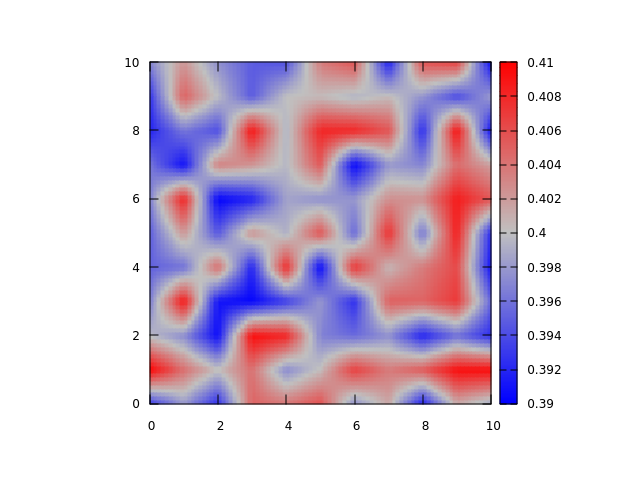
\includegraphics[width=1.0\linewidth]{initialper.png}
  \caption{t=0}
  \label{fig:sub1}
\end{subfigure}%
\begin{subfigure}{.5\textwidth}
  \centering
  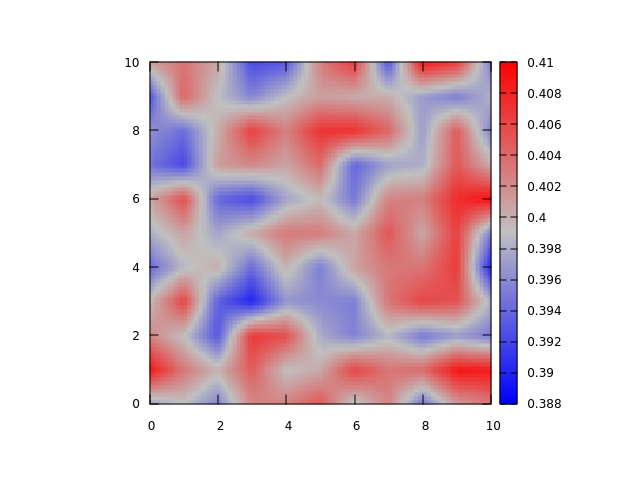
\includegraphics[width=1.0\linewidth]{30per.png}
  \caption{t=30dt}
  \label{fig:sub2}
\end{subfigure}
\label{fig:test}
\end{figure}


\begin{figure}
\centering
\begin{subfigure}{.5\textwidth}
  \centering
  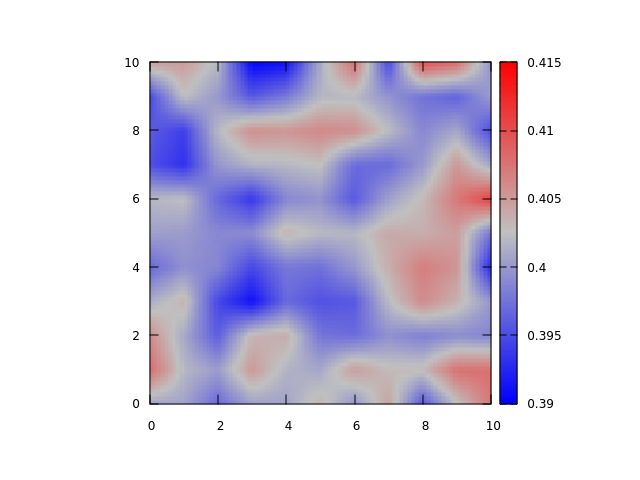
\includegraphics[width=1.0\linewidth]{100per.png}
  \caption{t=100dt}
  \label{fig:sub1}
\end{subfigure}%
\begin{subfigure}{.5\textwidth}
  \centering
  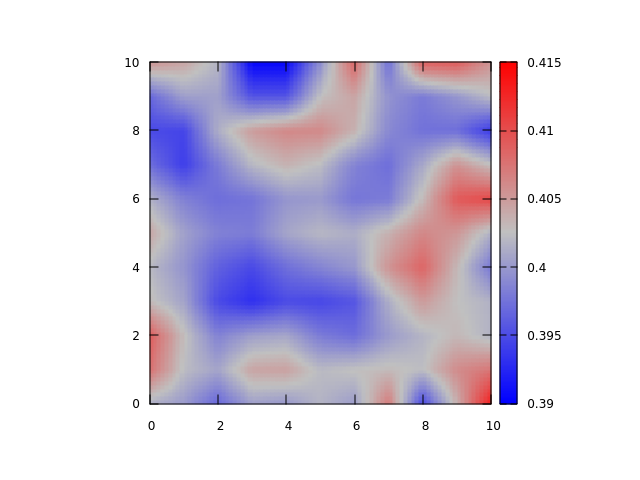
\includegraphics[width=1.0\linewidth]{500per.png}
  \caption{t=500dt}
  \label{fig:sub2}
\end{subfigure}
\label{fig:test}
\end{figure}
\vfill

\begin{figure}
\centering
\begin{subfigure}{.5\textwidth}
  \centering
  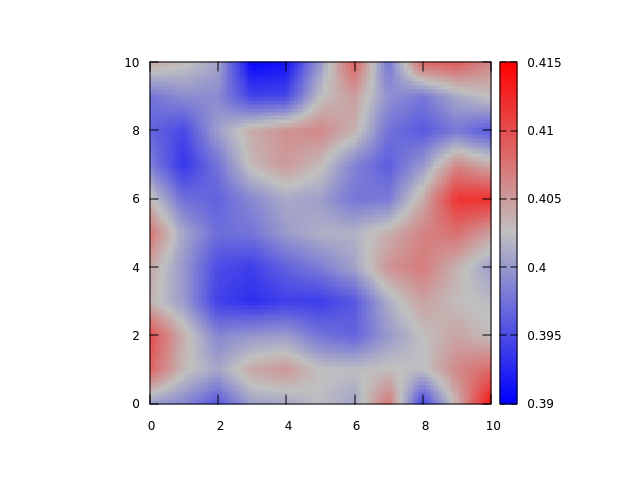
\includegraphics[width=1.0\linewidth]{1000per.png}
  \caption{t=1000dt}
  \label{fig:sub1}
\end{subfigure}%
\begin{subfigure}{.5\textwidth}
  \centering
  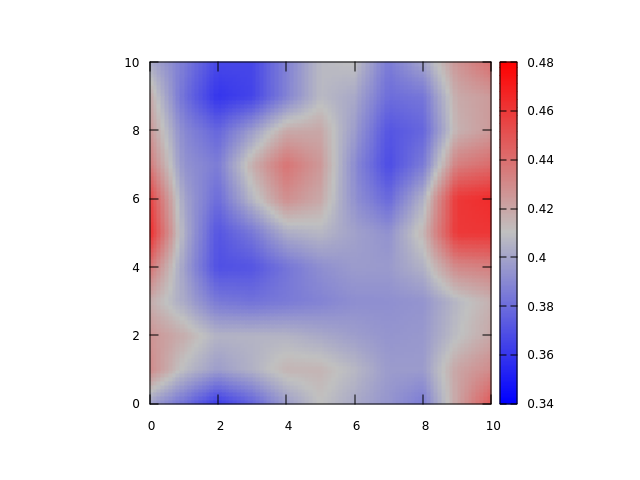
\includegraphics[width=1.0\linewidth]{5000per.png}
  \caption{t=5000dt}
  \label{fig:sub2}
\end{subfigure}
\label{fig:test}
\end{figure}

\vfill

\vfill
\clearpage

\section{Phase-field model for wetting phenomena}
\subsection{Statement of the problem}
Wetting phenomena typically involve a fluid-fluid interface advancing or receding on a solid substrate and a contact line
formed at the intersection between the interface and the substrate. The wetting properties of the substrate determine to a
large extent the behaviour of the fluids in the contact-line region. To account for wetting phenomena and contact lines on solid boundaries, the CH equation can be coupled to a
wall boundary condition [138]. Such models find applications in various situations, including microfluidic
devices  flow in porous media, rheological systems , and patterning of thin polymer films and others. Many
of these applications are characterised by the presence of chemically heterogeneous substrates and complex geometries,
which make their numerical simulation challenging.
Throughout this chapter, $\Omega \subset \mathbb{R}^2$ corresponds to a $2$-dimensional rectangular domain, $\partial \Omega$ denotes its boundary with outward unit normal vector $\mathbf{n}$, $\mathcal{S}$ is the solid substrate, and $\mathcal{G} = \partial \Omega \setminus \mathcal{S}$. The CH system we use to describe the dynamics of two immiscible fluids in contact with a solid substrate is a free-energy-based model. We consider systems with a free energy given by
\begin{equation}
E(\phi) := E_m(\phi) + E_w(\phi)
\end{equation}
where the two terms, $E_m$ and $E_w$, represent the mixing and wall components of the free energy, respectively. Here $F_m(\phi) = \frac{1}{4}(\phi^2 - 1)^2$, and $F_w$ is taken to be a cubic polynomial:
\begin{equation}
F_w(\phi) = \frac{\sqrt{2}}{2} \cos \theta(x)\left(\frac{\phi^3}{3} - \phi\right)
\end{equation}
where $\theta = \theta(x)$ is the equilibrium contact angle, which can depend on the spatial position $x$. From the expression of the free energy, we calculate that, for a sufficiently smooth function $\psi : \Omega \to \mathbb{R}$:
\begin{equation}
\frac{d}{d\alpha}E(\phi + \alpha\psi)\bigg|_{\alpha=0} = \int_{\Omega}\left(\frac{1}{\varepsilon}f_m(\phi) - \varepsilon\phi\right)\psi d\Omega + \int_{\partial \Omega}(f_w(\phi) + \varepsilon\nabla\phi \cdot \mathbf{n})\psi d\sigma
\end{equation}
with $f_m = F_m'$ and $f_w = F_w'$, so the chemical potential is equal to
\begin{equation}
\mu := \frac{\delta E}{\delta \phi} = \frac{1}{\varepsilon}f_m(\phi) - \varepsilon\phi
\end{equation}
and the natural boundary condition associated with the surface energy is
\begin{equation}
\varepsilon\nabla\phi \cdot \mathbf{n} = -f_w(\phi) = \frac{\sqrt{2}}{2} \cos \theta(x)(1 - \phi^2)
\end{equation}
We assume that the dynamics of the system is governed by the CH equation,
\begin{equation}
\frac{\partial\phi}{\partial t} = \nabla \cdot (b(x) \nabla\mu)
\end{equation}
where $b(x)$ is a mobility parameter, assumed to be equal to one. The mass-conservation property holds:
\begin{equation}
\frac{d}{dt}M(\phi) := \frac{d}{dt}\int_{\Omega}\phi d\Omega = \int_{\partial \Omega}\nabla\mu \cdot \mathbf{n}d\sigma
\end{equation}
The mass flux at the boundary can be specified enforcing certain condition on $\nabla\mu \cdot.$ In particular, we will set $\nabla\mu = 0$ at the solid boundary, $\mathcal{S}$. The system becomes:
\begin{align}
\frac{\partial\phi}{\partial t} &= \nabla \cdot ( \nabla\mu) \\
\mu &= \frac{1}{\varepsilon}f_m(\phi) - \varepsilon \Delta{\phi}, \quad x \in \Omega, t \in (0, T] \\
\varepsilon\nabla\phi \cdot \mathbf{n} &= -f_w(\phi) \\
\nabla\mu \cdot \mathbf{n} &= 0, \quad x \in \partial\Omega, t \in (0, T]
\end{align}
\subsection{The weak formulation}
The weak formulation of equations (141) to~(145) is as follows: find $(\phi, \mu)$ such that
\begin{equation}
\begin{aligned}
    \phi &\in L^{\infty}(0, T; H^1(\Omega)), \\
    \frac{\partial\phi}{\partial t} &\in L^2(0, T; (H^1(\Omega))'), \\
    \mu &\in L^2(0, T; H^1(\Omega)),
\end{aligned}
\end{equation}
and the following variational formulation is satisfied:
\begin{align}
    \langle \frac{\partial\phi}{\partial t}, \psi \rangle + ( \nabla\mu, \nabla\psi) &= 0, \quad \forall \psi \in H^1(\Omega) \text{ and almost everywhere for t in}\quad (0,T], \label{eq:variational1} \\
    (\mu, \eta) &= \varepsilon (\nabla\phi, \nabla\eta) + \frac{1}{\varepsilon} (f_m(\phi), \eta) + (f_w(\phi), \eta)_{\partial\Omega}, \quad \forall \eta \in H^1(\Omega) \text{ and almost everywhere for t in}\quad (0,T] \label{eq:variational2}
\end{align}

\subsection{The temporal discretization and the algorithm}
For the problem of this chapter we opt again for a standard backward Euler scheme that can be combined with some convex splitting scheme for the potential term to ensure unconditionall stability and convergence as shown in the first chapter. For a more recent review of new numerical schemes proposed for the wetting phenomena that arise in the context of the Cahn Hilliard equation we refer to \ref{AYMARD2019100010}. As shown in the previous chapters we have to handle a nonlinear system of equations on each timepoint using the Newton-Raphson method. One difference of the implementation aspect of the problem has to do with the boundary integral term:
\begin{align}
\int_{\partial\Omega}\eta(1-\phi^2)ds
\end{align}
 arising from the wall energy. For the cases we examine we have a simple form for this term as our domain is a rectangle and we know explicitly the normal vector on each side. This new term has to be added to the residual vector and is calculated as a sum of contibutions of four integral terms each one representing the integration on the corresponding boundary line (bottom,right,top,left):
 \begin{align}
\int_{\partial\Omega}\eta(1-\phi^2)ds = \int_{\partial\Omega_{b}}\eta(1-\phi^2)ds + \int_{\partial\Omega_{r}}\eta(1-\phi^2)ds + \int_{\partial\Omega_{t}}\eta(1-\phi^2)ds +\int_{\partial\Omega_{l}}\eta(1-\phi^2)ds
\end{align}
  Each of these four integrals is calculated as a sum over the elements whose one side intersects the corresponding boundary line:
\begin{align}
\int_{\partial\Omega_{l}}\eta(1-\phi^2)ds = \sum_{e}\int_{\partial\Omega_{e}}\eta(1-\phi^2)ds,\quad \text{where}\quad {\partial\Omega_{e}}\cap l \neq \emptyset
\end{align}
   The AssembleSystem subroutine shows the required modifications.
   
\subsubsection{Results}
Here, we study the coalescence of two adjacent sessile droplets as they spread on a flat substrate. For the simulation, we used the initial condition:

\[
\phi(x,y,0) = 1 - \tanh \left( \frac{\sqrt{(x - x_1)^2 + y^2} - r^2}{\sqrt{2\varepsilon}} \right) - \tanh \left( \frac{\sqrt{(x - x_2)^2 + y^2} - r^2}{\sqrt{2\varepsilon}} \right)
\]

in the domain \([0, 2] \times [0, 0.5]\), with \(x_1 = 0.65\), \(x_2 = 1.35\), \(r = 0.25\), and at the boundary, we imposed a uniform contact angle, \(\theta = \pi/4\), using the wall energy.
The results that follow show the evolution of the phase field during the simulation. Here $e=10^-1$ and the timpestep was considered fixed $ dt = 5\times10^-7$ and $10^4$ steps where forced.

\vfill
\begin{figure}
\centering
\begin{subfigure}{.5\textwidth}
  \centering
  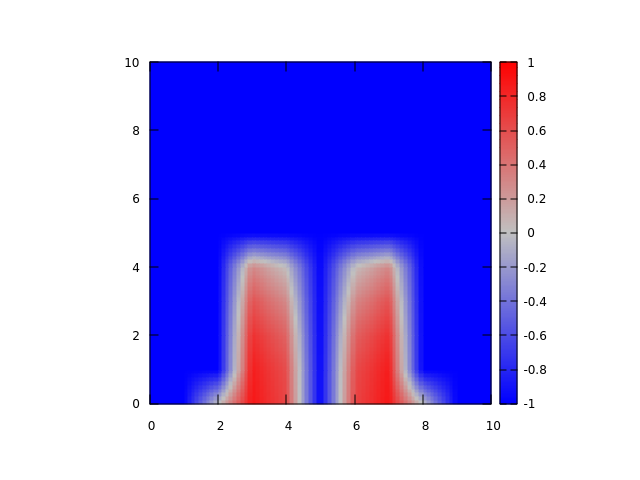
\includegraphics[width=1.0\linewidth]{initialcontact.png}
  \caption{t=0}
  \label{fig:sub1}
\end{subfigure}%
\begin{subfigure}{.5\textwidth}
  \centering
  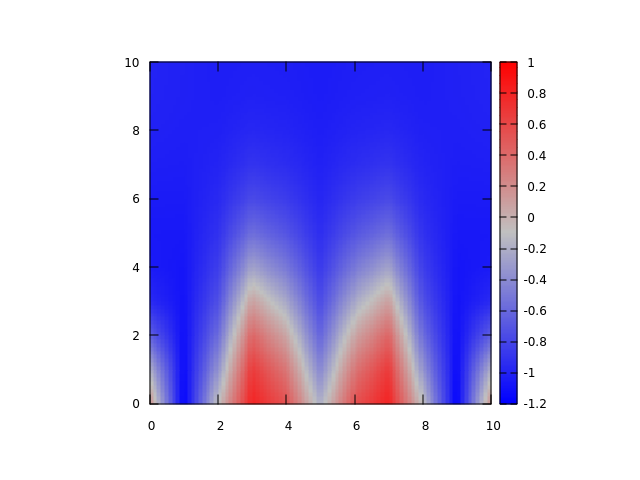
\includegraphics[width=1.0\linewidth]{1000contact.png}
  \caption{t=1000dt}
  \label{fig:sub2}
\end{subfigure}
\label{fig:test}
\end{figure}


\begin{figure}
\centering
\begin{subfigure}{.5\textwidth}
  \centering
  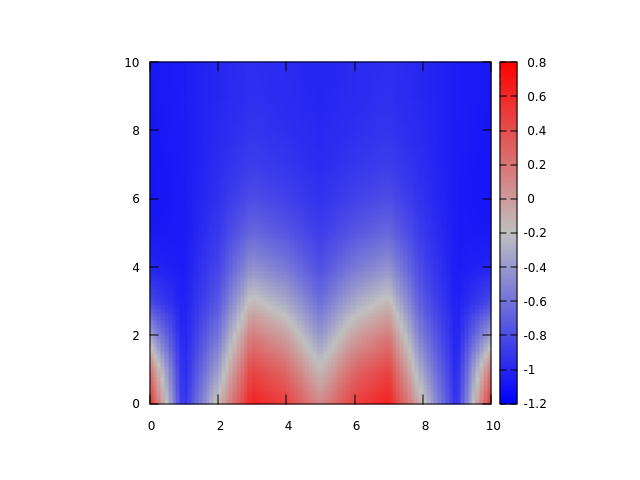
\includegraphics[width=1.0\linewidth]{3000contact.png}
  \caption{t=3000dt}
  \label{fig:sub1}
\end{subfigure}%
\begin{subfigure}{.5\textwidth}
  \centering
  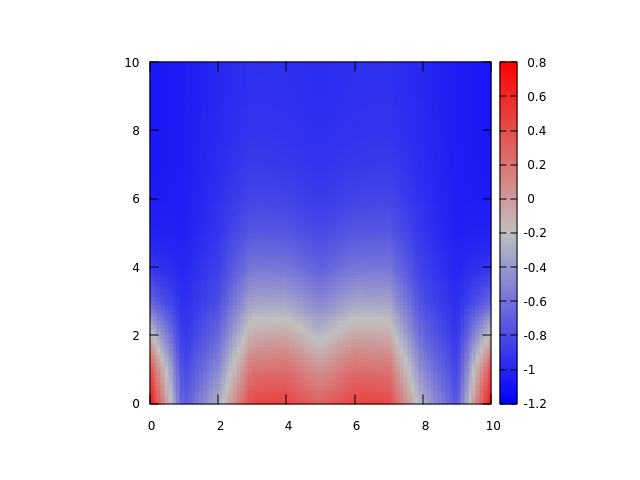
\includegraphics[width=1.0\linewidth]{6000contact.png}
  \caption{t=6000dt}
  \label{fig:sub2}
\end{subfigure}
\label{fig:test}
\end{figure}
\vfill

\begin{figure}
\centering
\begin{subfigure}{.5\textwidth}
  \centering
  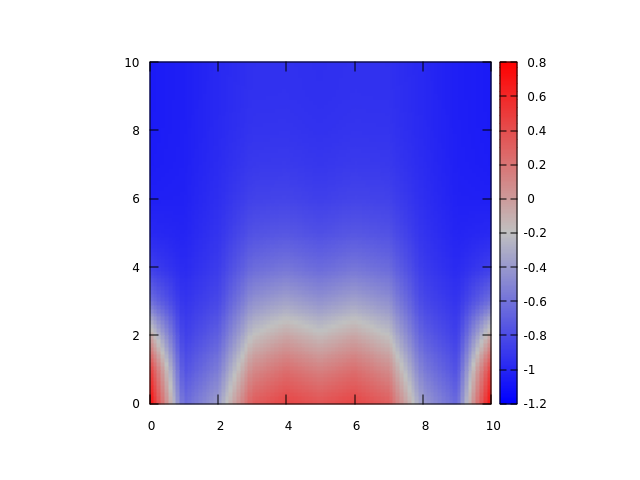
\includegraphics[width=1.0\linewidth]{8000contact.png}
  \caption{t=8000dt}
  \label{fig:sub1}
\end{subfigure}%
\begin{subfigure}{.5\textwidth}
  \centering
  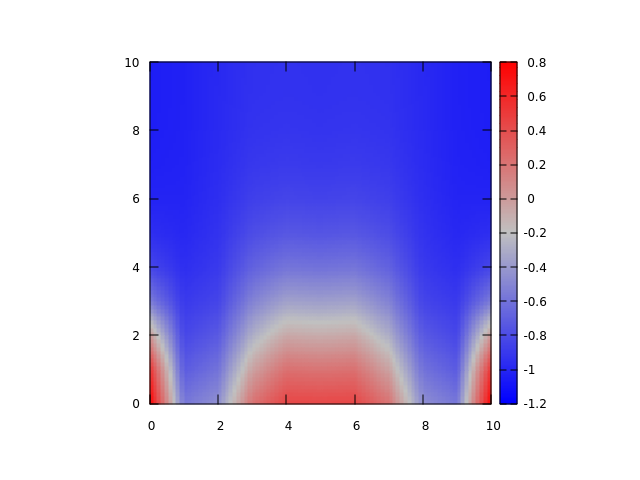
\includegraphics[width=1.0\linewidth]{10000contact.png}
  \caption{t=10000dt}
  \label{fig:sub2}
\end{subfigure}
\label{fig:test}
\end{figure}
\begin{figure}
\caption {Evolution of phase field for $\theta = \pi/4$ }
\end{figure}


\vfill



\clearpage
\newpage

\vfill
\begin{figure}
\centering
\begin{subfigure}{.5\textwidth}
  \centering
  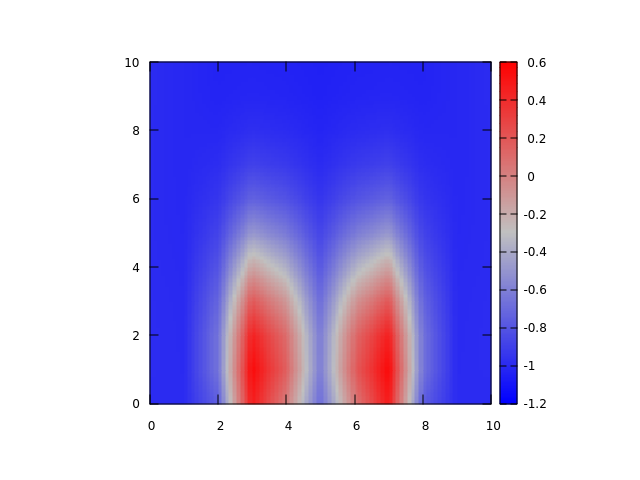
\includegraphics[width=1.0\linewidth]{1000contact3p4.png}
  \caption{t=1000dt}
  \label{fig:sub1}
\end{subfigure}%
\begin{subfigure}{.5\textwidth}
  \centering
  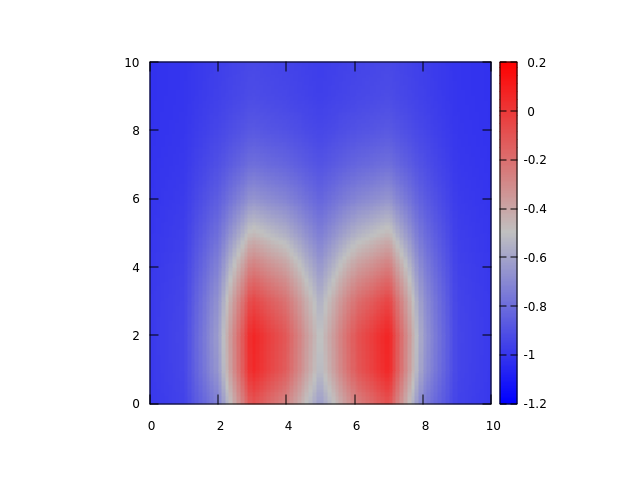
\includegraphics[width=1.0\linewidth]{3000contact3p4.png}
  \caption{t=000dt}
  \label{fig:sub2}
\end{subfigure}
\label{fig:test}
\end{figure}

\begin{figure}
\centering
\begin{subfigure}{.5\textwidth}
  \centering
  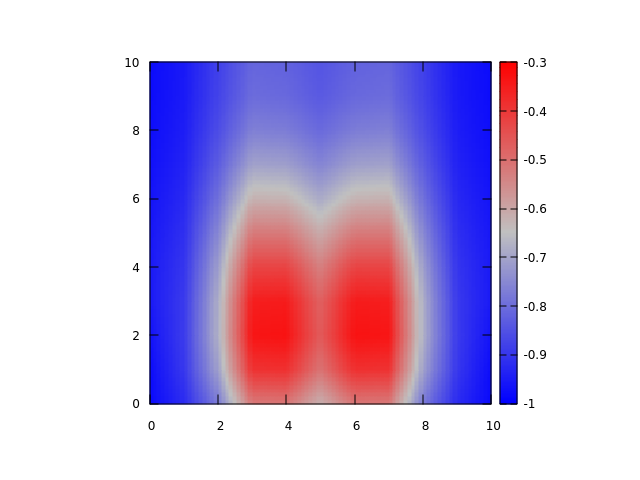
\includegraphics[width=1.0\linewidth]{6000contact3p4.png}
  \caption{t=6000dt}
  \label{fig:sub1}
\end{subfigure}%
\begin{subfigure}{.5\textwidth}
  \centering
  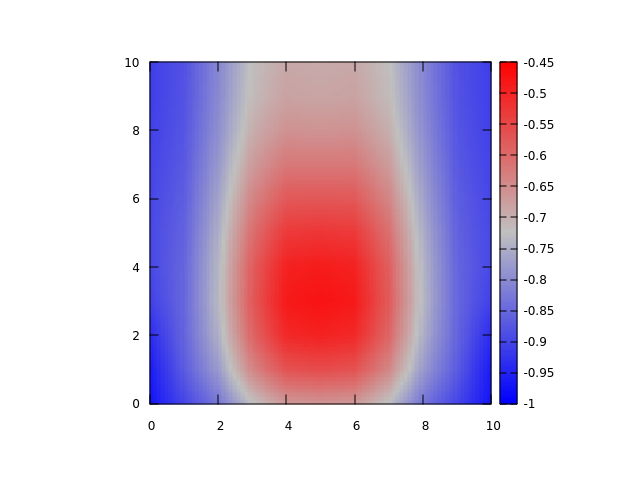
\includegraphics[width=1.0\linewidth]{10000contact3p4.png}
  \caption{t=10000dt}
  \label{fig:sub2}
\end{subfigure}
\label{fig:test}
\end{figure}
\begin{figure}
\caption {Evolution of phase field for $\theta = 3\pi/4$ }
\end{figure}



\vfill
\clearpage

\newpage


\section{The implementation}
This chapter is devoted to the implementation aspects for the boundary value problems examined in the previous sections. The source code is written in FORTRAN, and it implements a backward Euler method with minor modifications, like convex splitting, or midpoint approximation of the chemical potential, and/or modifications on the standard Ginzburg-Landau potential for some runs. We opt for a fixed timepoint approach that has to be chosen accordingly to the remarks made for the stability/unique-solvabitlity and convergence that are noted in the temporal dicretization section of this work. For the better presentation of the implementation aspects, we consider three main programs named respectively: NEUMANN.f90, PERIODIC.f90 and CONTACTANGLE.f90 .

\subsection{Dependencies}
The \texttt{NEUMANN/PERIODIC/CONTACTANGLE} programs relie on the following dependencies:
\begin{itemize}
    \item \texttt{iso\_fortran\_env}: Intrinsic module providing essential Fortran environment parameters.
    \item \texttt{BiCGStab\_mod}: A custom module containing the BiCGStab solver implementation.
    \item \texttt{PARAMETERS\_NEUMANN/PERIODIC/CONTACTANGLE.inc}: An included configuration file that sets program parameters.
\end{itemize}

\subsection{Program Components}
The \texttt{NEUMANN/PERIODIC/CONTACTANGLE} programs consist of various components, including:

\subsection{Space and Time Coordinates}
The program initializes space coordinates \texttt{x} and \texttt{y} for the simulation. These coordinates define the spatial domain over which the problem is solved. Additionally, it sets up time coordinates \texttt{t} to track the simulation's progression.

\subsection{Local to Global Node Numbering}
The \texttt{nop} array represents local to global node connectivity list, allowing for the mapping of local node indices to global node indices. This mapping is crucial for assembling the system of equations.

\subsection{Order Parameter Variables}
The program handles the order parameter, denoted as \texttt{u}, which corresponds to the Cahn-Hilliard equation's primary variable. It manages both \texttt{u\_new} and \texttt{u\_old} variables for tracking the solution's evolution over time.

\subsection{Chemical Potential Variables}
An auxiliary variable, denoted as \texttt{w}, represents the chemical potential. Similar to the order parameter, it manages both \texttt{w\_new} and \texttt{w\_old} variables.

\subsection{Newton Tolerance Parameters}
The program defines tolerance parameters for the Newton-Raphson method, including \texttt{tolS} for the convergence tolerance, \texttt{ntrial} for the maximum number of Newton iterations, and \texttt{max\_iter} for the maximum number of iterations allowed in the BiCGStab solver.

\subsection{Stationary System of Newton Cycle}
The \texttt{fvec} and \texttt{fjac} arrays represent the equation systems used in the Newton-Raphson iterations. These arrays contain the system's right-hand side (RHS) and the Jacobian matrix. To improve computational efficiency, the arrays are divided into four components: \texttt{fjac1}, \texttt{fjac2}, \texttt{fjac3}, and \texttt{fjac4}.

\subsection{Local Contributions}
Local contributions from each element are accumulated into \texttt{fjac1}, \texttt{fjac2}, \texttt{fjac3}, and \texttt{fjac4}. Similarly, \texttt{fvec1} and \texttt{fvec2} store the local contributions to the right-hand side of the equation system.

\subsection{Newton Solution Vector}
The \texttt{dSol} array represents the correction vector obtained from the Newton-Raphson iterations. It is added to the solution vector \texttt{Sol} to update the solution.

\subsection{Loop Variables}
The program uses various loop variables, including \texttt{element}, \texttt{timepoint}, \texttt{trial}, \texttt{n}, \texttt{m}, and \texttt{L}. These variables control the program's flow and iteration.

\subsection{Convergence Check}
A boolean variable, \texttt{CONVERGENT}, is used to check for convergence within the Newton-Raphson loop. The program stops iterating when convergence is achieved or after reaching the maximum number of iterations.

\subsection{File Handling}
The program reads and writes data to files. The \texttt{OPEN}, \texttt{WRITE}, and \texttt{CLOSE} statements are used for file handling.

\subsection{Program Execution}
The execution of the \texttt{NEUMANN/PERIODIC/CONTACTANGLE} programs involves several steps:

\begin{enumerate}
    \item Import the required dependencies, including \texttt{iso\_fortran\_env}, \texttt{BiCGStab\_mod}, and \texttt{PARAMETERS\_NEUMANN/PERIODIC/CONTACTANGLE.inc}.
    \item Initialize space and time coordinates (\texttt{x}, \texttt{y}, and \texttt{t}).
    \item Perform local-to-global node numbering (\texttt{nop}).
    \item Set the initial conditions for the order parameter (\texttt{u\_old} and \texttt{u\_new}) and the chemical potential (\texttt{w\_old} and \texttt{w\_new}).
    \item Enter a time loop to simulate the problem at various time points.
    \item For each time point, perform a Newton-Raphson iteration to improve the solution.
    \item Check for convergence within the Newton-Raphson loop.
    \item Write results to output files at specified intervals.
\end{enumerate}

\section{NEUMANN.f90}
This subsection contains the main routine executed and an optionary modification to a linear problem suggested by Provatas and Elder and popularized by Eyre and as subsections the subroutines employed.
\begin{verbatim}
program NEUMANN
    use, intrinsic :: iso_fortran_env
    USE BiCGStab_mod
    IMPLICIT NONE
    INCLUDE 'PARAMETERS_NEUMANN.inc'
 
    !> Space coordinates
    REAL(real64) x(NNmax),y(NNmax)
 
    !> Time coordinates
    REAL(real64) t(Tmax)
 
    !> Local to global node numbering
    INTEGER nop(NELmax,NNref)

    !> Order parameter - u - of the Cahn Hilliard Equation
    REAL(real64) u_new(NNmax)
    REAL(real64) u_old(NNmax)

    !> Auxiliary variable - w - the chemical potential
    REAL(real64) w_new(NNmax)
    REAL(real64) w_old(NNmax)
 
    !> Newton tolerance parameters
    REAL(real64),PARAMETER:: tolS=1.0E-5_real64
    INTEGER, PARAMETER :: ntrial = 100
    INTEGER, PARAMETER :: max_iter = 1000
 
    !> Stationary system of Newton cycle
    REAL(real64) fvec(2*NNmax)
    REAL(real64) fjac(2*NNmax,2*NNmax)

    !> Local contributions
    REAL(real64) fjac1(NNmax,NNmax)
    REAL(real64) fjac2(NNmax,NNmax)
    REAL(real64) fjac3(NNmax,NNmax)
    REAL(real64) fjac4(NNmax,NNmax)
    
    REAL(real64) fvec1(NNmax)
    REAL(real64) fvec2(NNmax)
 
    !> Newton solution vector
    REAL(real64) dSol(2*NNmax)
    REAL(real64) Sol(2*NNmax)
 
 
    INTEGER element,timepoint,trial,n,m,L
    LOGICAL CONVERGENT
    CHARACTER(10) :: timepoint_str

    OPEN(unit=1,file='initial_NEUMANN.dat')

    WRITE(*,'(25x,A)') 'Results c(n,t)'
    CALL SpaceDiscretization(x,y)
    CALL GlobalNodeNumbering(nop)
 
    !> Set time grid
    t=0.0_real64
    CALL TimeDiscretization(t)
 
    !>****************************************************************
    !> Set the initial conditions for the c,w variables of the problem
    !> For timepoint = 1
    !>*****************************************************************
    u_old=0.0_real64
    u_new=0.0_real64
    w_old=0.0_real64
    w_new=0.0_real64
    CALL InitialConditions(x,y,u_old,u_new,w_old,w_new)
    DO n=1,NNx
       WRITE(1,*) (u_old((n-1)*NNy+m),m=1,NNy)
    ENDDO
    CLOSE(1)
   
  !>**********************************************************************************
  !> Given an initial guess x for a root in n dimensions, take ntrial Newton-Raphson
  !> steps to improve the root. Stop if the root converges in either summed absolute
  !> variable increments tolx or summed absolute function values tolf.
  !>**********************************************************************************
 
 !> Time loop to attain the solution at every timepoint
    DO timepoint=2,Tmax
       print *, "Time point: ", timepoint
 
       trial=0
       CONVERGENT=.false.
       Sol=0.0_real64

       !> Choose the initial guess for the first newton iteration
       Sol(1:NNmax) = w_old(:) 
       Sol(NNmax+1:2*NNmax) = u_old(:) 
 
       !> Start the Newton iteration loop
       DO WHILE (.NOT.CONVERGENT .AND. trial < ntrial)
          dSol=0.0_real64
          
          !>******************************************************************
          !> Set the Stationary System to be solved at every Newton iteration
          !> ___________________Fjac.dx = -Fvec_______________________________
          !>******************************************************************
          fvec=0.0_real64
          fjac=0.0_real64

          fjac1=0.0_real64
          fjac2=0.0_real64
          fjac3=0.0_real64
          fjac4=0.0_real64

          fvec1=0.0_real64
          fvec2=0.0_real64

          !> Local contributions
          DO element=1,NELmax
          CALL AssembleSystem(x,y,element,nop,u_old,u_new,w_new,w_old,fjac1,fjac2,fjac3,fjac4,fvec1,fvec2)
          ENDDO

         !> Global system 
         fvec(1:NNmax) = fvec1(:)
         fvec(NNmax+1:2*NNmax) = fvec2(:)

         fjac(1:NNmax,1:NNmax) = fjac1(:,:)
         fjac(1:NNmax,NNmax+1:2*NNmax) = fjac2(:,:)
         fjac(NNmax+1:2*NNmax,1:NNmax) = fjac3(:,:)
         fjac(NNmax+1:2*NNmax,NNmax+1:2*NNmax) = fjac4(:,:)

          !> Solve the system - find the correction dSol
          fvec = -fvec
          dSol = BiCGStab(fjac,fvec)
          
          !> Update the solution
          Sol(:) = Sol(:) + dSol(:)
         
          !> Check for convergence
          CONVERGENT = (NORM2(fvec) < tolS)
          print*,"CONVERGENCE", CONVERGENT
 
          trial = trial + 1
          w_new(:) = Sol(1:NNmax)
          u_new(:) = Sol(NNmax+1:2*NNmax)
          
         ENDDO  !> Newton trial loop
         
         IF (CONVERGENT) THEN
            u_old(:) = u_new(:)
            w_old(:) = w_new(:)
          write(*,*) 'Newton-Raphson converged in', trial, 'iterations'

       !> Write the results
          IF ((timepoint<=100 .and. MOD(timepoint,10)==0).or.MOD(timepoint, 50) == 0) THEN
            
            WRITE(timepoint_str, '(I0)') timepoint  ! Convert the integer to a string
          
            OPEN(UNIT=2, FILE=TRIM(ADJUSTL(timepoint_str)) // '_NEUMANN.dat')
            DO n = 1, NNx
              WRITE(2, *) (u_new((n - 1) * NNy + m), m = 1, NNy)
            ENDDO
          
            CLOSE(2)
          ENDIF
          

       ELSE
          write(*,*) 'Newton-Raphson did not converge within', ntrial, 'iterations'
       ENDIF
    ENDDO !> Time loop

   !>*************************************************************
   !> FORWARD EULER & PROVATAS/ELDER 2010
   !>*************************************************************  
   !  DO timepoint=2,Tmax
   !    print*,'timepoint',timepoint
   !    Sol=0.0_real64
   !>*****************************************************************
   !> Calculate the double well potential and the derivative
   !> Depend on c, the order parameter
   !>*****************************************************************
         !  f=0.0_real64
         !  J=0.0_real64
         !  DO element=1,NELmax
         !     CALL PotentialTerm(x,y,element,nop,timepoint,c,f,J)
         !  ENDDO

         !  fvec=0.0_real64
         !  fjac=0.0_real64
         ! CALL StationarySystem(timePoint,c,w,STIFF,MASS,f,J,fjac,fvec)
 
         !  !> Solve the system - find the correction dSol
         !  Sol = BiCGStab(fjac,fvec)

         !   w(:,timepoint) = Sol(1:NNmax)
         !   c(:,timepoint) = Sol(NNmax+1:2*NNmax)

         ! ENDDO !TIME LOOP     

END program NEUMANN
\end{verbatim}

\subsection{Space Discretization}
\begin{verbatim}
SUBROUTINE SpaceDiscretization(x,y)
    use, intrinsic :: iso_fortran_env
    IMPLICIT NONE
    INCLUDE 'PARAMETERS_NEUMANN.inc'
 
    !> Space coordinates
    REAL(real64) x(NNmax),y(NNmax)
 
    REAL(real64) xorigin,yorigin,xlast,ylast
    REAL(real64) dx,dy
    INTEGER i,j,NNode
 
    x=0.0_real64
    y=0.0_real64
 
    xorigin=0.0_real64
    xlast=1.0_real64
    dx=(xlast-xorigin)/real(2*NELx)
 
    yorigin=0.0_real64
    ylast=1.0_real64
    dy=(ylast-yorigin)/real(2*NELy)
 
    !> Setting the coordinates of each node
    x(1)=xorigin
    y(1)=yorigin
    DO i=1,NNx
       NNode = (i-1)*NNy + 1 ! Ascending node numbering from bottom left up to right
       x(NNode) = x(1) + (i-1)*dx
       y(NNode) = y(1)
       DO j=2,NNy
          x(NNode+j-1)=x(NNode)
          y(NNode+j-1)=y(NNode)+(j-1)*dy
       ENDDO
    ENDDO
END SUBROUTINE SpaceDiscretization
\end{verbatim}
\subsection{Global Node Numbering}
\begin{verbatim}
SUBROUTINE GlobalNodeNumbering(nop)
    use, intrinsic :: iso_fortran_env
    IMPLICIT NONE
    INCLUDE 'PARAMETERS_NEUMANN.inc'
 
    !> Local to global space numbering
    INTEGER nop(NELmax,NNref)
 
    INTEGER i,j,k,l,NEL
    NEL=0
    DO i=1,NELx
       DO j=1,NELy
          NEL=NEL+1
          DO k=1,3
             l=3*k-2
             nop(nel,l)=nny*(2*i+k-3)+2*j-1
             nop(nel,l+1)=nop(nel,l)+1
             nop(nel,l+2)=nop(nel,l)+2
          ENDDO
       ENDDO
    ENDDO
 END SUBROUTINE GlobalNodeNumbering
\end{verbatim}
\subsection{Time Discretization}
\begin{verbatim}
SUBROUTINE TimeDiscretization(t)
    use, intrinsic :: iso_fortran_env
    IMPLICIT NONE
    INCLUDE 'PARAMETERS_NEUMANN.inc'
 
    !> Time coordinates
    REAL(real64) t(Tmax)
 
    REAL(real64)  Tinit
 
    INTEGER j
 
    Tinit=0.0_real64
 
 
    t(1)=Tinit
    DO j=2,Tmax
       t(j) = (j-1)*dt
    ENDDO
 
 END SUBROUTINE TimeDiscretization
\end{verbatim}

\subsection{Initial Conditions}
\begin{verbatim}
SUBROUTINE InitialConditions(x, y, u_old,u_new,w_old,w_new)
    use, intrinsic :: iso_fortran_env
    IMPLICIT NONE
    INCLUDE 'PARAMETERS_NEUMANN.inc'
 
    !> Space coordinates
    REAL(real64), DIMENSION(NNmax) :: x, y
 
    !> Order parameter - c - of the Cahn Hilliard Equation
    REAL(real64), DIMENSION(NNmax) :: u_old
    REAL(real64), DIMENSION(NNmax) :: u_new
 
    !> Auxiliary variable - w - the chemical potential
    REAL(real64), DIMENSION(NNmax) :: w_old
    REAL(real64), DIMENSION(NNmax) :: w_new
 
    INTEGER :: i,n,m

 
 
    DO i = 1, NNmax

      CALL RANDOM_NUMBER(u_old(i))
      !u_old(i) = 0.63_real64 + 0.02_real64*(0.5_real64-u_old(i))
      u_old(i) = 2.0_real64*u_old(i)-1.0_real64
      w_old(i) = 0.0_real64
    

    ENDDO

  
 
 END SUBROUTINE InitialConditions
\end{verbatim}

\subsection{The system of each Newton cycle}
This subroutine assembles the stationary system that is to be solved on every Newton iteration. Some different options for the potential and for the numerical scheme that are contained in comments, could be inserted in a parametric form in a more refined version of the code.
\begin{verbatim}
SUBROUTINE AssembleSystem(x,y,element,nop,u_old,u_new,w_new,w_old,fjac1,fjac2,fjac3,fjac4,fvec1,fvec2)
   use, intrinsic :: iso_fortran_env
   IMPLICIT NONE
   INCLUDE 'PARAMETERS_NEUMANN.inc'



   !> Space coordinates !xpt,ypt
   REAL(real64), INTENT(IN) :: x(NNmax),y(NNmax)

   !> Current element
   INTEGER element

   !> Local to global space numbering
   INTEGER nop(NELmax,NNref)
   INTEGER ngl(NNref)

   !> Order parameter - c - of the Cahn Hilliard Equation
   REAL(real64) u_new(NNmax)
   REAL(real64) u_old(NNmax)
   REAL(real64) w_new(NNmax)
   REAL(real64) w_old(NNmax)
 

 
   !> Local contributions
   REAL(real64) fjac1(NNmax,NNmax)
   REAL(real64) fjac2(NNmax,NNmax)
   REAL(real64) fjac3(NNmax,NNmax)
   REAL(real64) fjac4(NNmax,NNmax)
   
   REAL(real64) fvec1(NNmax)
   REAL(real64) fvec2(NNmax)



   REAL(real64) phi(NNref), tphx(NNref), tphy(NNref),phic(NNref),phie(NNref)
   REAL(real64) gp(3), gw(3)
   REAL(real64) Xdomain,Xc,Xe,Ydomain,Yc,Ye,dett

   REAL(real64) u0i,ui,ux,uy,wi,wx,w0x,wy,w0y
   INTEGER i,r,k,l,m,n



   gw  =(/0.27777777777778, 0.444444444444, 0.27777777777778/)
   gp =(/0.1127016654    , 0.5           , 0.8872983346    /)

   DO i = 1,NNref
      ngl(i) = nop(element,i)
   ENDDO

   ! Loop over qauss points
   DO r = 1,3
      DO k = 1,3

         call TestFunctions(gp(r),gp(k),phi,phic,phie)

         ! Defines the domain domain coordinates and the 2-dimensional Jacobian dett
         Xdomain=0.0_real64
         Xc=0.0_real64
         Xe=0.0_real64
         Ydomain=0.0_real64
         Yc=0.0_real64
         Ye=0.0_real64
         DO n=1,NNref
            Xdomain= Xdomain + x(ngl(n)) * phi(n)
            Xc= Xc + x(ngl(n)) * phic(n)
            Xe= Xe + x(ngl(n)) * phie(n)
            Ydomain= Ydomain + y(ngl(n)) * phi(n)
            Yc= Yc + y(ngl(n)) * phic(n)
            Ye= Ye + y(ngl(n)) * phie(n)
         ENDDO
         dett=Xc*Ye-Xe*Yc

         DO i=1,NNref
            tphx(i)=(Ye*phic(i)-Yc*phie(i))/dett
            tphy(i)=(Xc*phie(i)-Xe*phic(i))/dett
         ENDDO

         u0i = 0.0_real64
         ui = 0.0_real64
         ux = 0.0_real64
         uy = 0.0_real64
         wi = 0.0_real64
         wx = 0.0_real64
         w0x = 0.0_real64
         wy = 0.0_real64
         w0y = 0.0_real64
         DO i=1,NNref
            u0i = u0i + u_old(ngl(i))*phi(i)
            ui = ui + u_new(ngl(i))*phi(i) 
            ux = ux + u_new(ngl(i))*tphx(i)
            uy = uy + u_new(ngl(i))*tphy(i)
         ENDDO
         DO i=1,NNref
            wi = wi + w_new(ngl(i))*phi(i) 
            wx = wx + w_new(ngl(i))*tphx(i)
            w0x = w0x + w_old(ngl(i))*tphx(i)
            wy = wy + w_new(ngl(i))*tphy(i)
            w0y = w0y + w_old(ngl(i))*tphy(i)
         ENDDO
         
        !*********************************
        !W = 100c**2(1-c)**2 FENICS
        !*********************************  
         ! DO l=1,NNref
         !   f(ngl(l)) = f(ngl(l)) + gw(r)*gw(k)*dett*(100.0)*(ui**2)*(( 1.0 - ui)**2)*phi(l)
         !    DO m=1,NNref
         !       J(ngl(l),ngl(m)) =  J(ngl(l),ngl(m)) + gw(r)*gw(k)*dett*(200.0)*(ui*(1.0-ui)*(1.0-2.0*ui))*phi(l)*phi(m)
         !    ENDDO
         ! ENDDO

        !***************************************************
        !W = 0.25(c**2-1)**2 ginzburg landau 
        !*************************************************** 
        !  DO l=1,NNref
        !    f(ngl(l)) = f(ngl(l)) + gw(r)*gw(k)*dett*(ui**3 - ui)*phi(l)
        !    DO m=1,NNref
        !       J(ngl(l),ngl(m)) =  J(ngl(l),ngl(m)) + gw(r)*gw(k)*dett*((3.0_real64)*(ui**2) - 1.0_real64)*phi(l)*phi(m)
        !    ENDDO
        ! ENDDO
        
        !****************************************************
        !W = 0.25(c**2-1)**2 ginzburg landau & convex splitting
        !**************************************************** 
        ! DO l=1,NNref
        !    f(ngl(l)) = f(ngl(l)) + gw(r)*gw(k)*dett*(ui**3)*phi(l)
        !    DO m=1,NNref
        !       J(ngl(l),ngl(m)) =  J(ngl(l),ngl(m)) + gw(r)*gw(k)*dett*((3.0_real64)*(ui**2))*phi(l)*phi(m)
        !    ENDDO
        ! ENDDO

         
         DO l=1,NNref
            
            fvec1(ngl(l)) = fvec1(ngl(l)) + gw(r)*gw(k)*dett*wi*phi(l) -gw(r)*gw(k)*dett*(100.0_real64)*(2.0_real64*ui - 6.0_real64*ui**2 + 4.0_real64*ui**3 )*phi(l) &
            -(e)**2*gw(r)*gw(k)*dett*(ux*tphx(l)+uy*tphy(l))
           
              fvec2(ngl(l)) = fvec2(ngl(l)) + gw(r)*gw(k)*dett*ui*phi(l) - gw(r)*gw(k)*dett*u0i*phi(l) &
              + 0.5*(dt)*gw(r)*gw(k)*dett*(wx*tphx(l)+wy*tphy(l)) + 0.5*(dt)*gw(r)*gw(k)*dett*(w0x*tphx(l)+w0y*tphy(l)) !theta fenics
              
           DO m=1,NNref
              
                 fjac1(ngl(l),ngl(m)) = fjac1(ngl(l),ngl(m)) + gw(r)*gw(k)*dett*phi(l)*phi(m)
              
                 fjac2(ngl(l),ngl(m)) = fjac2(ngl(l),ngl(m)) -(e)**2*gw(r)*gw(k)*dett*(tphx(l)*tphx(m)+tphy(l)*tphy(m)) &
                 - gw(r)*gw(k)*dett*(100.0_real64)*((2.0_real64 - 12.0_real64*ui+ 12.0_real64*ui**2))*phi(l)*phi(m)
              
                 fjac3(ngl(l),ngl(m)) = fjac3(ngl(l),ngl(m)) + (dt)*gw(r)*gw(k)*dett*(tphx(l)*tphx(m)+tphy(l)*tphy(m))
              
                 fjac4(ngl(l),ngl(m)) = fjac4(ngl(l),ngl(m)) + gw(r)*gw(k)*dett*phi(l)*phi(m)
                  
            ENDDO
         ENDDO   
      ENDDO
   ENDDO


END SUBROUTINE AssembleSystem
 
\end{verbatim}

\subsection{The test functions}
\begin{verbatim}
SUBROUTINE TestFunctions(x,y,phi,phic,phie)
    use, intrinsic :: iso_fortran_env
    IMPLICIT NONE
    INCLUDE 'PARAMETERS_NEUMANN.inc'
 
    !> Point at which to form the test functions
    REAL(real64),DIMENSION(NNref):: phi,phic,phie
    REAL(real64), INTENT(IN) :: x,y
    REAL(real64) ::  l1x, l2x, l3x, l1y, l2y, l3y
    REAL(real64) :: dl1x,dl2x,dl3x, dl1y, dl2y, dl3y
 
    !*** One Statement Functions ***
    l1x=2.*x**2-3.*x+1.
    l2x=-4.*x**2+4.*x
    l3x=2.*x**2-x
    dl1x=4.*x-3.
    dl2x=-8.*x+4.
    dl3x=4.*x-1.
 
    l1y=2.*y**2-3.*y+1.
    l2y=-4.*y**2+4.*y
    l3y=2.*y**2-y
    dl1y=4.*y-3.
    dl2y=-8.*y+4.
    dl3y=4.*y-1.
    !*******************************
 
    phi(1)=l1x*l1y
    phi(2)=l1x*l2y
    phi(3)=l1x*l3y
    phi(4)=l2x*l1y
    phi(5)=l2x*l2y
    phi(6)=l2x*l3y
    phi(7)=l3x*l1y
    phi(8)=l3x*l2y
    phi(9)=l3x*l3y
    phic(1)=l1y*dl1x
    phic(2)=l2y*dl1x
    phic(3)=l3y*dl1x
    phic(4)=l1y*dl2x
    phic(5)=l2y*dl2x
    phic(6)=l3y*dl2x
    phic(7)=l1y*dl3x
    phic(8)=l2y*dl3x
    phic(9)=l3y*dl3x
    phie(1)=l1x*dl1y
    phie(2)=l1x*dl2y
    phie(3)=l1x*dl3y
    phie(4)=l2x*dl1y
    phie(5)=l2x*dl2y
    phie(6)=l2x*dl3y
    phie(7)=l3x*dl1y
    phie(8)=l3x*dl2y
    phie(9)=l3x*dl3y
 
 END SUBROUTINE TestFunctions
\end{verbatim}

\section{PERIODIC.f90}
For the implementation of the periodic conditions we show only the essential modifications that the systems matrices/vectors undergo when we impose the conditions under the analysis stated in the relevant chapter of this work. After the system is assembled as in the Neumann case the corresponding left-right and top-bottom node lines/rows of the system matrices are added, setting zero the residual on the right and top nodes and setting one to the systems Jacobian. Also a recovery of the boundary values for the right and top nodes follows after each iteration.

\begin{verbatim}
program PERIODIC
    use, intrinsic :: iso_fortran_env
    USE BiCGStab_mod
    IMPLICIT NONE
    INCLUDE 'PARAMETERS_PERIODIC.inc'
 
    !> Space coordinates
    REAL(real64) x(NNmax),y(NNmax)
 
    !> Time coordinates
    REAL(real64) t(Tmax)
 
    !> Local to global node numbering
    INTEGER nop(NELmax,NNref)
 
    !> Order parameter - u - of the Cahn Hilliard Equation
    REAL(real64) u_new(NNmax)
    REAL(real64) u_old(NNmax)

 
    !> Auxiliary variable - w - the chemical potential
    REAL(real64) w_new(NNmax)
    REAL(real64) w_old(NNmax)
   
 
    !> Newton tolerance parameters
    REAL(real64),PARAMETER:: tolS=1.0E-5_real64
    INTEGER, PARAMETER :: ntrial = 100
    INTEGER, PARAMETER :: max_iter = 1000
 
    !> Stationary system of Newton cycle
    REAL(real64) fvec(2*NNmax)
    REAL(real64) fjac(2*NNmax,2*NNmax)
    !> Local contributions
    REAL(real64) fjac1(NNmax,NNmax)
    REAL(real64) fjac2(NNmax,NNmax)
    REAL(real64) fjac3(NNmax,NNmax)
    REAL(real64) fjac4(NNmax,NNmax)
    
    REAL(real64) fvec1(NNmax)
    REAL(real64) fvec2(NNmax)
 
    !> Newton solution vector
    REAL(real64) dSol(2*NNmax)
    REAL(real64) Sol(2*NNmax)

    INTEGER element,timepoint,trial,n,m,l
    LOGICAL CONVERGENT
    CHARACTER(10) :: timepoint_str
 
    OPEN(unit=1,file='initial_PERIODIC.dat')

    
 
    WRITE(*,'(25x,A)') 'Results c(n,t)'
    CALL SpaceDiscretization(x,y)
    CALL GlobalNodeNumbering(nop)
 
 
    !> Set time grid
    t=0.0_real64
    CALL TimeDiscretization(t)
 
    !>****************************************************************
    !> Set the initial conditions for the c,w variables of the problem
    !> For timepoint = 1
    !>*****************************************************************
    u_old=0.0_real64
    u_new=0.0_real64
    w_old=0.0_real64
    w_new=0.0_real64
    CALL InitialConditions(x,y,u_old,u_new,w_old,w_new)

    DO n=1,NNx
       WRITE(1,*) (u_old((n-1)*NNy+m),m=1,NNy)
    ENDDO
    CLOSE(1)

    
     !>***********************************************************************************
     !> Given an initial guess x for a root in n dimensions, take ntrial Newton-Raphson
     !> steps to improve the root. Stop if the root converges in either summed absolute
     !> variable increments tolx or summed absolute function values tolf.
     !>***********************************************************************************

 
   !> Time loop to attain the solution at every timepoint
    DO timepoint=2,Tmax
      print *, "Time point: ", timepoint

      trial=0
      CONVERGENT=.false.
      Sol=0.0_real64


      
      !> Choose the initial guess for the first newton iteration
      Sol(1:NNmax) = w_old(:) 
      Sol(NNmax+1:2*NNmax) = u_old(:) 
      
      !> Start the Newton iteration loop
      DO WHILE (.NOT.CONVERGENT .AND. trial < ntrial)
         dSol=0.0_real64

         !>******************************************************************
         !> Set the Stationary System to be solved at every Newton iteration
         !> ___________________Fjac.dx = -Fvec_______________________________
         !>******************************************************************
          fvec=0.0_real64
          fjac=0.0_real64

          fjac1=0.0_real64
          fjac2=0.0_real64
          fjac3=0.0_real64
          fjac4=0.0_real64

          fvec1=0.0_real64
          fvec2=0.0_real64

          !> Local contributions
          DO element=1,NELmax
          CALL AssembleSystem(x,y,element,nop,u_old,u_new,w_new,fjac1,fjac2,fjac3,fjac4,fvec1,fvec2)
          ENDDO
          !> Global system 
          fvec(1:NNmax) = fvec1(:)
          fvec(NNmax+1:2*NNmax) = fvec2(:)

         fjac(1:NNmax,1:NNmax) = fjac1(:,:)
         fjac(1:NNmax,NNmax+1:2*NNmax) = fjac2(:,:)
         fjac(NNmax+1:2*NNmax,1:NNmax) = fjac3(:,:)
         fjac(NNmax+1:2*NNmax,NNmax+1:2*NNmax) = fjac4(:,:)

         !> Imposing the periodic conditions
         DO l=1,NNy 
            fvec(l) = fvec(l) + fvec(NNmax-NNy+l)
            fvec(NNmax-NNy+l) = 0.0_real64 

            fjac(l,:) = fjac(l,:) + fjac(NNmax-NNy+l,:)
            fjac(:,l) = fjac(:,l) + fjac(:,NNmax-NNy+l)
            fjac(NNmax-NNy+l,:) = 0.0_real64
            fjac(:,NNmax-NNy+l) = 0.0_real64
            fjac(NNmax-NNy+l,NNmax-NNy+l) = 1.0_real64
         ENDDO        
         DO l=2,NNx-1 
            fvec((l-1)*NNy+1) = fvec((l-1)*NNy+1) + fvec(l*NNy)
            fvec(l*NNy) = 0.0_real64 

            fjac((l-1)*NNy+1,:) = fjac((l-1)*NNy+1,:) + fjac(l*NNy,:)
            fjac(:,(l-1)*NNy+1) = fjac(:,(l-1)*NNy+1) + fjac(:,l*NNy)
            fjac(l*NNy,:) = 0.0_real64
            fjac(:,l*NNy) = 0.0_real64
            fjac(l*NNy,l*NNy) = 1.0_real64
         ENDDO        

         !> Solve the system - find the correction dSol
         fvec = -fvec
         dSol = BiCGStab(fjac,fvec)
         
         !> Recover the right boundary nodes
         DO l=1,NNy 
            dSol(NNmax-NNy+l) = dSol(l)
            dsol(2*NNmax-NNy+l) = dSol(NNmax+l)
         ENDDO 
         !> Recover the top nodes  
         DO l=2,NNx-1 
            dSol(l*NNy) = dSol((l-1)*NNy+1)
            dsol(NNmax+l*NNy) = dSol(NNmax+(l-1)*NNy+1)
         ENDDO 

         !> Update the solution
         Sol(:) = Sol(:) + dSol(:)

         DO l=1,2*NNmax
            IF (Sol(l) <= - 0.9999) THEN 
               Sol(l) = - 0.9999 
            ELSEIF (Sol(l) >= 0.9999) THEN 
               Sol(l) = 0.9999
            ENDIF   
         ENDDO   
     
         !> Check for convergence
         CONVERGENT = (NORM2(dSol) < tolS)
         print*,"CONVERGENCE", CONVERGENT

         trial = trial + 1
         w_new(:) = Sol(1:NNmax)
         u_new(:) = Sol(NNmax+1:2*NNmax)

      ENDDO  !> Newton trial loop
      
      IF (CONVERGENT) THEN

               u_old(:) = u_new(:)
               w_old(:) = w_new(:)

         write(*,*) 'Newton-Raphson converged in', trial, 'iterations'


         IF ((timepoint<=100 .and. MOD(timepoint,10)==0).or.MOD(timepoint, 500) == 0) THEN
            
            WRITE(timepoint_str, '(I0)') timepoint  ! Convert the integer to a string
          
            OPEN(UNIT=2, FILE=TRIM(ADJUSTL(timepoint_str)) // '_PERIODIC.dat')
            DO n = 1, NNx
              WRITE(2, *) (u_new((n - 1) * NNy + m), m = 1, NNy)
            ENDDO
          
            CLOSE(2)
          ENDIF

      

      ELSE
         write(*,*) 'Newton-Raphson did not converge within', ntrial, 'iterations'
      ENDIF


   ENDDO !> Time loop

 END program PERIODIC
\end{verbatim}
\section{CONTACTANGLE.f90}
For the wetted wall conditions to be examined in this program the essential modifications concern the AssembleSystem subroutine, to take into account the wall energy term. For this purpose the first lines of this subroutine are modified to calculate the boundary integral term arising from the weak formulation.
\begin{verbatim}
SUBROUTINE AssembleSystem(x,y,element,BoundaryElement,BottomElement,RightElement,TopElement,LeftElement,nop,&
   u_old,u_new,w_new,fjac1,fjac2,fjac3,fjac4,fvec1,fvec2,flux,dflux)
   use, intrinsic :: iso_fortran_env
   IMPLICIT NONE
   INCLUDE 'PARAMETERS_CONTACT.inc'



   !> Space coordinates !xpt,ypt
   REAL(real64), INTENT(IN) :: x(NNmax),y(NNmax)

   !> Current element
   INTEGER element
    !> Location indices to check for Boundary Elements
   INTEGER BottomElement(NELmax)
   INTEGER RightElement(NELmax)
   INTEGER TopElement(NELmax)
   INTEGER LeftElement(NELmax)

   !> Boundary element control index
   INTEGER BoundaryElement(NELmax)

   !> Local to global space numbering
   INTEGER nop(NELmax,NNref)
   INTEGER ngl(NNref)

   !> Order parameter - c - of the Cahn Hilliard Equation
   REAL(real64) u_new(NNmax)
   REAL(real64) u_old(NNmax)
   REAL(real64) w_new(NNmax)
 

 
   !> Local contributions
   REAL(real64) fjac1(NNmax,NNmax)
   REAL(real64) fjac2(NNmax,NNmax)
   REAL(real64) fjac3(NNmax,NNmax)
   REAL(real64) fjac4(NNmax,NNmax)
   
   REAL(real64) fvec1(NNmax)
   REAL(real64) fvec2(NNmax)

   REAL(real64) flux(NNmax)
   REAL(real64) fluxb(NNmax)
   REAL(real64) fluxr(NNmax)
   REAL(real64) fluxt(NNmax)
   REAL(real64) fluxl(NNmax)

   REAL(real64) Dflux(NNmax,NNmax)
   REAL(real64) Dfluxb(NNmax,NNmax)
   REAL(real64) Dfluxr(NNmax,NNmax)
   REAL(real64) Dfluxt(NNmax,NNmax)
   REAL(real64) Dfluxl(NNmax,NNmax)



   REAL(real64) phi(NNref), tphx(NNref), tphy(NNref),phic(NNref),phie(NNref)
   REAL(real64) gp(3), gw(3)
   REAL(real64) Xdomain,Xc,Xe,Ydomain,Yc,Ye,dett

   REAL(real64) u0i,ui,ux,uy,wi,wx,wy
   INTEGER i,j,r,k,l,m,n



   gw  =(/0.27777777777778, 0.444444444444, 0.27777777777778/)
   gp =(/0.1127016654    , 0.5           , 0.8872983346    /)

   DO i = 1,NNref
      ngl(i) = nop(element,i)
   ENDDO

   
   fluxb=0.0_real64
   fluxr=0.0_real64
   fluxt=0.0_real64
   fluxl=0.0_real64
   
   Dfluxb=0.0_real64
   Dfluxr=0.0_real64
   Dfluxt=0.0_real64
   Dfluxl=0.0_real64

   IF (BoundaryElement(element)==1) THEN

      !> check which side of the boundary the element belongs to
      IF (BottomElement(element)==1)THEN
         DO j=1,3
            CALL TestFunctions(gp(j),0.0_real64,phi, phic, phie)

            Xdomain=0.0_real64
            Xc=0.0_real64
            Xe=0.0_real64
            Ydomain=0.0_real64
            Yc=0.0_real64
            Ye=0.0_real64
            DO n=1,NNref
               Xdomain= Xdomain + x(ngl(n)) * phi(n)
               Xc= Xc + x(ngl(n)) * phic(n)
               Xe= Xe + x(ngl(n)) * phie(n)
               Ydomain= Ydomain + y(ngl(n)) * phi(n)
               Yc= Yc + y(ngl(n)) * phic(n)
               Ye= Ye + y(ngl(n)) * phie(n)
            ENDDO
            dett=Xc*Ye-Xe*Yc

            DO i=1,NNref
               tphx(i)=(Ye*phic(i)-Yc*phie(i))/dett
               tphy(i)=(Xc*phie(i)-Xe*phic(i))/dett
            ENDDO

            ui = 0.0_real64
            ux = 0.0_real64
            uy = 0.0_real64
            DO i=1,NNref
               ui = ui + u_new(ngl(i))*phi(i)
               ux = ux + u_new(ngl(i))*tphx(i)
               uy = uy + u_new(ngl(i))*tphy(i)
            ENDDO
            

            DO m=1,7,3
               fluxb(ngl(m)) = fluxb(ngl(m)) + gw(j)*dett*(1.0_real64-ui**2)*phi(m)
            ENDDO  
            
            DO l=1,7,3
               DO m=1,7,3
                  Dfluxb(ngl(l),ngl(m)) = Dfluxb(ngl(l),ngl(m)) +gw(j)*dett*(- 2.0_real64*ui*phi(m))*phi(l)
               ENDDO 
            ENDDO        
         ENDDO

      IF (RightElement(element)==1)THEN
         DO j=1,3
            CALL TestFunctions(1.0_real64,gp(j),phi, phic, phie)

            Xdomain=0.0_real64
            Xc=0.0_real64
            Xe=0.0_real64
            Ydomain=0.0_real64
            Yc=0.0_real64
            Ye=0.0_real64
            DO n=1,NNref
               Xdomain= Xdomain + x(ngl(n)) * phi(n)
               Xc= Xc + x(ngl(n)) * phic(n)
               Xe= Xe + x(ngl(n)) * phie(n)
               Ydomain= Ydomain + y(ngl(n)) * phi(n)
               Yc= Yc + y(ngl(n)) * phic(n)
               Ye= Ye + y(ngl(n)) * phie(n)
            ENDDO
            dett=Xc*Ye-Xe*Yc

            DO i=1,NNref
               tphx(i)=(Ye*phic(i)-Yc*phie(i))/dett
               tphy(i)=(Xc*phie(i)-Xe*phic(i))/dett
            ENDDO

            ui = 0.0_real64
            ux = 0.0_real64
            uy = 0.0_real64
            DO i=1,NNref
               ui = ui + u_new(ngl(i))*phi(i)
               ux = ux + u_new(ngl(i))*tphx(i)
               uy = uy + u_new(ngl(i))*tphy(i)
            ENDDO



            DO m=7,9              
                  fluxr(ngl(m)) = fluxr(ngl(m)) +gw(j)*dett*(1.0_real64-ui**2)*phi(m)
            ENDDO

            DO l=7,9
               DO m=7,9
                  Dfluxr(ngl(l),ngl(m)) = Dfluxr(ngl(l),ngl(m)) + gw(j)*dett*(- 2.0_real64*ui*phi(m))*phi(l)
               ENDDO 
            ENDDO        
         ENDDO

      ELSEIF (TopElement(element)==1)THEN
         DO j=1,3
            CALL TestFunctions(gp(j),1.0_real64,phi, phic, phie)

            Xdomain=0.0_real64
            Xc=0.0_real64
            Xe=0.0_real64
            Ydomain=0.0_real64
            Yc=0.0_real64
            Ye=0.0_real64
            DO n=1,NNref
               Xdomain= Xdomain + x(ngl(n)) * phi(n)
               Xc= Xc + x(ngl(n)) * phic(n)
               Xe= Xe + x(ngl(n)) * phie(n)
               Ydomain= Ydomain + y(ngl(n)) * phi(n)
               Yc= Yc + y(ngl(n)) * phic(n)
               Ye= Ye + y(ngl(n)) * phie(n)
            ENDDO
            dett=Xc*Ye-Xe*Yc

            DO i=1,NNref
               tphx(i)=(Ye*phic(i)-Yc*phie(i))/dett
               tphy(i)=(Xc*phie(i)-Xe*phic(i))/dett
            ENDDO

            ui = 0.0_real64
            ux = 0.0_real64
            uy = 0.0_real64
            DO i=1,NNref
               ui = ui + u_new(ngl(i))*phi(i)
               ux = ux + u_new(ngl(i))*tphx(i)
               uy = uy + u_new(ngl(i))*tphy(i)
            ENDDO

            DO m=3,9,3             
                  fluxt(ngl(m)) = fluxt(ngl(m)) + gw(j)*dett*(1.0_real64-ui**2)*phi(m)
            ENDDO

            DO l=3,9,3
               DO m=3,9,3
                  Dfluxt(ngl(l),ngl(m)) = Dfluxt(ngl(l),ngl(m)) + gw(j)*dett*(- 2.0_real64*ui*phi(m))*phi(l)
               ENDDO 
            ENDDO        
         ENDDO

      ELSEIF (LeftElement(element)==1)THEN
         DO j=1,3
            CALL TestFunctions(0.0_real64,gp(j),phi, phic, phie)

            Xdomain=0.0_real64
            Xc=0.0_real64
            Xe=0.0_real64
            Ydomain=0.0_real64
            Yc=0.0_real64
            Ye=0.0_real64
            DO n=1,NNref
               Xdomain= Xdomain + x(ngl(n)) * phi(n)
               Xc= Xc + x(ngl(n)) * phic(n)
               Xe= Xe + x(ngl(n)) * phie(n)
               Ydomain= Ydomain + y(ngl(n)) * phi(n)
               Yc= Yc + y(ngl(n)) * phic(n)
               Ye= Ye + y(ngl(n)) * phie(n)
            ENDDO
            dett=Xc*Ye-Xe*Yc

            DO i=1,NNref
               tphx(i)=(Ye*phic(i)-Yc*phie(i))/dett
               tphy(i)=(Xc*phie(i)-Xe*phic(i))/dett
            ENDDO

            ui = 0.0_real64
            ux = 0.0_real64
            uy = 0.0_real64
            DO i=1,NNref
               ui = ui + u_new(ngl(i))*phi(i)
               ux = ux + u_new(ngl(i))*tphx(i)
               uy = uy + u_new(ngl(i))*tphy(i)
            ENDDO


            DO m=1,3
                  fluxl(ngl(m)) = fluxl(ngl(m)) + gw(j)*dett*(1.0_real64-ui**2)*phi(m)
            ENDDO

            DO l=1,3
               DO m=1,3
                  Dfluxl(ngl(l),ngl(m)) = Dfluxl(ngl(l),ngl(m)) + gw(j)*dett*(- 2.0_real64*ui*phi(m))*phi(l)
               ENDDO 
            ENDDO        
         ENDDO


      ENDIF
   ENDIF

   !> Summation of the components to the total FLUX
   DO l=1,NNref
      flux(ngl(l)) =  fluxb(ngl(l)) + fluxr(ngl(l)) + fluxt(ngl(l)) + fluxl(ngl(l))  
      DO m=1,NNref
         Dflux(ngl(l),ngl(m)) = Dflux(ngl(l),ngl(m)) &
         + Dfluxb(ngl(l),ngl(m)) + Dfluxr(ngl(l),ngl(m)) + Dfluxt(ngl(l),ngl(m)) + Dfluxl(ngl(l),ngl(m))
      ENDDO
   ENDDO      
   ! Loop over qauss points
 
ENDIF

   ! Loop over qauss points
   DO r = 1,3
      DO k = 1,3

         call TestFunctions(gp(r),gp(k),phi,phic,phie)

         ! Defines the domain domain coordinates and the 2-dimensional Jacobian dett
         Xdomain=0.0_real64
         Xc=0.0_real64
         Xe=0.0_real64
         Ydomain=0.0_real64
         Yc=0.0_real64
         Ye=0.0_real64
         DO n=1,NNref
            Xdomain= Xdomain + x(ngl(n)) * phi(n)
            Xc= Xc + x(ngl(n)) * phic(n)
            Xe= Xe + x(ngl(n)) * phie(n)
            Ydomain= Ydomain + y(ngl(n)) * phi(n)
            Yc= Yc + y(ngl(n)) * phic(n)
            Ye= Ye + y(ngl(n)) * phie(n)
         ENDDO
         dett=Xc*Ye-Xe*Yc

         DO i=1,NNref
            tphx(i)=(Ye*phic(i)-Yc*phie(i))/dett
            tphy(i)=(Xc*phie(i)-Xe*phic(i))/dett
         ENDDO

         u0i = 0.0_real64
         ui = 0.0_real64
         ux = 0.0_real64
         uy = 0.0_real64
         wi = 0.0_real64
         wx = 0.0_real64
         wy = 0.0_real64
         DO i=1,NNref
            u0i = u0i + u_old(ngl(i))*phi(i)
            ui = ui + u_new(ngl(i))*phi(i) 
            ux = ux + u_new(ngl(i))*tphx(i)
            uy = uy + u_new(ngl(i))*tphy(i)
         ENDDO
         DO i=1,NNref
            wi = wi + w_new(ngl(i))*phi(i) 
            wx = wx + w_new(ngl(i))*tphx(i)
            wy = wy + w_new(ngl(i))*tphy(i)
         ENDDO
         
        !*********************************
        !W = 100c**2(1-c)**2 FENICS
        !*********************************  
         ! DO l=1,NNref
         !   f(ngl(l)) = f(ngl(l)) + gw(r)*gw(k)*dett*(100.0)*(ui**2)*(( 1.0 - ui)**2)*phi(l)
         !    DO m=1,NNref
         !       J(ngl(l),ngl(m)) =  J(ngl(l),ngl(m)) + gw(r)*gw(k)*dett*(200.0)*(ui*(1.0-ui)*(1.0-2.0*ui))*phi(l)*phi(m)
         !    ENDDO
         ! ENDDO

        !***************************************************
        !W = 0.25(c**2-1)**2 ginzburg landau 
        !*************************************************** 
        !  DO l=1,NNref
        !    f(ngl(l)) = f(ngl(l)) + gw(r)*gw(k)*dett*(ui**3 - ui)*phi(l)
        !    DO m=1,NNref
        !       J(ngl(l),ngl(m)) =  J(ngl(l),ngl(m)) + gw(r)*gw(k)*dett*((3.0_real64)*(ui**2) - 1.0_real64)*phi(l)*phi(m)
        !    ENDDO
        ! ENDDO
        
        !****************************************************
        !W = 0.25(c**2-1)**2 ginzburg landau & convex splitting
        !**************************************************** 
        ! DO l=1,NNref
        !    f(ngl(l)) = f(ngl(l)) + gw(r)*gw(k)*dett*(ui**3)*phi(l)
        !    DO m=1,NNref
        !       J(ngl(l),ngl(m)) =  J(ngl(l),ngl(m)) + gw(r)*gw(k)*dett*((3.0_real64)*(ui**2))*phi(l)*phi(m)
        !    ENDDO
        ! ENDDO

         DO l=1,NNref
            
            fvec1(ngl(l)) = fvec1(ngl(l)) + gw(r)*gw(k)*dett*wi*phi(l) -(1.0_real64/e)*gw(r)*gw(k)*dett*(ui**3 - ui)*phi(l) &
             -(e)*gw(r)*gw(k)*dett*(ux*tphx(l)+uy*tphy(l)) +(sqrt(2.0_real64)/2.0_real64)*cos(theta)*flux(ngl(l))
            
               fvec2(ngl(l)) = fvec2(ngl(l)) + gw(r)*gw(k)*dett*ui*phi(l) - gw(r)*gw(k)*dett*u0i*phi(l) &
               + (dt)*gw(r)*gw(k)*dett*(wx*tphx(l)+wy*tphy(l)) 
               
            DO m=1,NNref
               
                  fjac1(ngl(l),ngl(m)) = fjac1(ngl(l),ngl(m)) + gw(r)*gw(k)*dett*phi(l)*phi(m)
               
                  fjac2(ngl(l),ngl(m)) = fjac2(ngl(l),ngl(m)) -(e)*gw(r)*gw(k)*dett*(tphx(l)*tphx(m)+tphy(l)*tphy(m)) &
                  -(1.0_real64/e)* gw(r)*gw(k)*dett*((3.0_real64)*(ui**2) - 1.0_real64)*phi(l)*phi(m) +(sqrt(2.0_real64)/2.0_real64)*cos(theta)*Dflux(ngl(l),ngl(m))
               
                  fjac3(ngl(l),ngl(m)) = fjac3(ngl(l),ngl(m)) + (dt)*gw(r)*gw(k)*dett*(tphx(l)*tphx(m)+tphy(l)*tphy(m))
               
                  fjac4(ngl(l),ngl(m)) = fjac4(ngl(l),ngl(m)) + gw(r)*gw(k)*dett*phi(l)*phi(m)
                  
            ENDDO
         ENDDO   
      ENDDO
   ENDDO


END SUBROUTINE AssembleSystem
\end{verbatim}
\newpage
\section{Future directions for the development of the code}
The numerical methods for phase transition problems is a rich subject whose perspectives can be reflected on the future development directions of the current implementation. The main effort should focus on exploitting the second order schemes for the higher accuracy and for the better stability and solvability properties they present. Secondly one has to take into account that the different stages of the morphological evolution of the phase field occur at different time scales, indicating the need of an adaptive time step approach. For example, in the spinodal decomposition
simulation, an initial random perturbation evolves on a fast time scale and later coarsening evolves on a very slow time scale.
Therefore, if a uniform small time step is used to capture the fast dynamics, the computation is very costly. On the other
hand, if a uniform large time step is used, fast time evolutions may be overlooked. Hence, it is essential to use an adaptive
time step method to simulate phenomena with multiple time scales. Thirdly one has to take into account that "stiff" systems may occur and for these cases a wide range of preconditioning strategies can be employed to reduce the condition number of the system that has to be solved on each Newton cycle. For these strategies we refer to \cite{Wu2011PreconditionersFT} Along with these aspects, crucial would be the modification of the classical Newton-Raphson procedure, to an inexact iterative scheme or to a globally convergent process like the line search or the multidimensional secant method (Broyden's Method, etc). To improve the performance it would be mandatory to exploit techniques of the sparse matrix formulations replacing costly computations with more efficient matrix to vector action when needed, etc. Finally of a more contemporary significance would be the effort to couple these modifications with the flow equations, to develop a tool for the Cahn-Hilliard-Navier-Stokes problem. We illustarate briefly some of these directions.
\subsubsection{Adaptive time stepping}
For the general outline of the techniques presented in this chapter we follow \cite{LI20171855} and the references therein.
A proposed adaptive time-stepping method using a criterion related to a residual of the discrete energy law \begin{equation}
\frac{dE(\varphi)}{dt} = -\int_{\Omega} \left|\nabla\mu(x, t)\right|^2 \, dx.
\end{equation} is the following:\\
Given $\varphi_n$, $\varphi_{n-1}$, $1/t_n$, $1/t_{n-1}$, and a parameter $\theta > 1$, chosen to be $\theta = 1.1$, the method is as follows:

\textbf{Step 1.} Compute $\varphi_{n+1}$ and obtain
\begin{equation}
R_{n+1} := E(\varphi_{n+1}) - E(\varphi_n) \frac{1}{t_n} + \int_{\Omega} \left|\nabla\mu_{n+1}\right|^2 \, dx. (7)
\end{equation}

\textbf{Step 2.} If $\left|R_{n+1}\right| > \text{resmax}$, take $1/t_n = 1/t_n/\theta$ and go to Step 1.

\textbf{Step 3.} If $\left|R_{n+1}\right| < \text{resmin}$, take $1/t_{n+1} = \theta \cdot 1/t_n$.

Here, a trial and error choice of $\text{resmax}$ and $\text{resmin}$ was used.\\

An adaptive time-stepping method using the time derivative of the total energy was considered in \cite{ref18}; that is,
\begin{equation}
\Delta t = \max(\Delta t_{min}, \frac{\Delta t_{max}}{\sqrt{ \left(1 + \alpha \left|E'(t)\right|^2\right)}}), (8)
\end{equation}
where the constant $\alpha$ is chosen to regulate the adaptivity. A large value of $\left|E'(t)\right|$ leads to a small time step, whereas a small $\left|E'(t)\right|$ value yields a large time step.

The following adaptive time-stepping technique was developed in \cite{ref19}:

\textbf{Step 1.} Calculate $e = \frac{\left\|\varphi_{n+1}^{\text{BE}} - \varphi_{n+1}^{\alpha}\right\|_{\alpha}}{\left\|\varphi_{n+1}^{\alpha}\right\|_{\alpha}}$, where $\varphi_{n+1}^{\text{BE}}$ and $\varphi_{n+1}^{\alpha}$ are the numerical solutions using the backward Euler method and a second-order generalized-$\alpha$ method with $\Delta t^n$, respectively.

\textbf{Step 2.} If $e > \text{tol}$, then reset the time step size $\Delta t^n = \rho\sqrt{\frac{\text{tol}}{e}}\cdot\Delta t^n$ and return to Step 1, where $\rho = 0.9$ and $\text{tol} = 10^{-3}$ are used. Otherwise, set $\Delta t^{n+1} = \rho\sqrt{\frac{\text{tol}}{e}}\cdot\Delta t^n$.\\

To equally distribute the locally computable discretization error, the authors in \cite{ref20} proposed the following algorithm:

\textbf{Step 1.} The global relative time discretization error estimate is defined by
\begin{equation}
e = \frac{\left\|\varphi_{n+1} - \hat{\varphi}_{n+1}\right\}_{\Delta t^n}}{\max\left(\left\|\varphi_{n+1}\right\|, \left\|\hat{\varphi}_{n+1}\right\|\right)},
\end{equation}
where $\varphi_{n+1}$ and $\hat{\varphi}_{n+1}$ are the numerical solutions obtained by taking two time steps of size $\Delta t^n/2$ and a single time step of size $\Delta t^n$ from $\varphi_n$, respectively.

\textbf{Step 2.} If $e < e_{\text{MAX}}$, then set
\begin{equation}
\Delta t^{n+1} = \Delta t^n {\left( \frac{e_{\text{tol}}}{e}\right)}^{1/p},
\end{equation}
where $e_{\text{MAX}}$ is a target error tolerance and $p$ is the global convergence rate of the time-stepping algorithm being used. If $e \geq e_{\text{MAX}}$, then that time step is rejected and go to Step 1, and recalculated with halving, i.e., $\Delta t^n = \Delta t^n/2$.

Also the authors in \cite{ref21} suggest an adaptive time-stepping scheme based on the convergence behavior of Newton–Raphson iterations. 
\subsubsection{ Broyden’s Method}
One drawback of the classical Newton's method is that the Jacobian matrix calculations in many problems is expensive, or even not feasible. For this reason a series of methods under the general name of secant methods provide cheap approximations to the Jacobian. The most popular of these methods is Broyden’s method.

Let us denote the approximate Jacobian by $B$. Then the ith quasi-Newton step $\delta x_i$ is the solution of:

\[
B_i \cdot \delta x_i = -F_i 
\]

where $\delta x_i = x_{i+1} - x_i$ (cf. equation 9.7.3). The quasi-Newton or secant condition is that $B_{i+1}$ satisfies:

\[
B_{i+1} \cdot \delta x_i = \delta F_i 
\]

where $\delta F_i = F_{i+1} - F_i$. This is a generalization of the one-dimensional secant approximation to the derivative, $\delta F/\delta x$. However, the previous equation does not determine $B_{i+1}$ uniquely in more than one dimension.

Many different auxiliary conditions to pin down $B_{i+1}$ have been explored, but the best-performing algorithm in practice results from Broyden’s formula. This formula is based on the idea of getting $B_{i+1}$ by making the least change to $B_i$ consistent with the secant equation. Broyden showed that the resulting formula is:

\[
B_{i+1} = B_i + \frac{\delta F_i - B_i \cdot \delta x_i}{\delta x_i \cdot \delta x_i} \delta x_i \otimes \delta x_i \cdot \delta x_i \quad 
\]


Early implementations of Broyden’s method used the Sherman-Morrison formula, to invert the last equation  analytically:

\[
B_{i+1}^{-1} = B_i^{-1} + \frac{(\delta x_i - B_i^{-1} \cdot \delta F_i) \otimes \delta x_i \cdot B_i^{-1}}{\delta x_i \cdot B_i^{-1} \cdot \delta F_i} \quad 
\]

Then instead of solving exactly , for example, LU decomposition may be employed, to determine $\delta x_i = -B_i^{-1} \cdot F_i$ by matrix multiplication in $O(N^2)$ operations. 


Since $B$ is not the exact Jacobian, we are not guaranteed that $\delta x$ is a descent search direction. Thus, the line search algorithm can fail to return a suitable step if $B$ wanders far from the true Jacobian. In this case, we reinitialize $B$. Like the secant method in one dimension, Broyden’s method converges superlinearly once you get close enough to the root. Embedded in a global strategy, it is almost as robust as Newton’s method and often needs far fewer function evaluations to determine a zero. Note that the final value of $B$ is not always close to the true Jacobian at the root, even when the method converges.





\bibliographystyle{ieeetr}
\bibliography{references}
\end{document}












